\section{The General Circulation of the
Atmosphere}\label{chp:GeneralCirculation}

\subsection{Space-time splittings}\label{space-time-splittings}

The dominant shape of the global circulation suggest that some
understanding can be gained from splitting the physical fields in larger
and smaller portions using appropriate averages. At a first inspection
the flow is seen as a predominant circumpolar vortex with superposed
fluctuations in space and time. The longitudinal directions i also known
as the "zonal" direction, therefore the average over longitude is known
as the zonal averaging.

\subsection{Zonal means}\label{zonal-means}

The zonal mean of a quantity \(A\) is defined as the average over
longitudes. Commonly used symbols int he literature are the overbar
(\(\bar{u}\)) or square brackets ((\([u]\)), the first is most
frequently encountered in the theoretical and modeling literature
whereas the second is most commonly used in observational and
diagnostics works. In the following we will use brackets.

\[[A] = \frac{1}{2\pi}\int_0^{2\pi} A \, dx\]

so that the total field can be decomposed as

\[A = [A] + A^*\]

where \(A^*\) is the deviation from the zonal mean. The average has the
properties that \([[A]] = [A]\) and \([A^*]=0\).

When a streamfunction can be defined, the average zonal mean meridional
velocity is zero:

\[= \frac{1}{2\pi}\int_0^{2\pi} v \, dx=\frac{1}{2\pi}\int_0^{2\pi} \frac{\partial \psi}{\partial x} \, dx=0\]

This is a consequence of the more general result that the zonal mean of
any quantity that is a longitude derivative is zero.

\subsection{Time means}\label{time-means}

The time mean is defined simply as the average over a length of time.
Also in this case several common symbols are used, once again the
overbar or sometimes curly brackets, in the following we will use the
overbar

\[\bar{A} = \frac{1}{T}\int_0^{T} A \, dt\]

so that the total field is

\[A = \bar{A} + A'\]

The deviations from the zonal means are called "eddy" components. An
eddy that obeys a dispersion relation is a "wave".

\subsection{Higher order quantities}\label{Sect:Higher}

The averages can be used to decompose higher order quantities. For
instance using zonal means a quadratic correlation of the form \(A B\)
can be decomposed as

\[A B = ([A]+A^*)([B]+B^*) = A^*B^* + [A] B^*+ A^*[B] + [A][B]\]

taking a further zonal mean we get

{\[= [A^*B^*+ [A]B^* + A^*[B] + [A][B]] =  [A][B] + [A^*B^*]\]}

because the mix terms disappear as the average of the deviations is
zero.

We can refine the splitting by considering the time average splitting of
the zonal terms:

\[\begin{aligned}
= \bar{[A]} + [A]' \\
A^* = \bar{A}^* + A'^*
\end{aligned}\]

These terms represent the stationary symmetric circulation, the
transient symmetric circulation and the stationaty deviation from the
zonal means ("asymmetries") and the transient asymmetries.

Inserting these relations into Eq.(\texttt{AB1}) we get

\[= (\bar{[A]} + [A]')(\bar{[B]} + [B]') + [A^*B^*]\]

the time mean of the terms linear in the time deviation will average
again to zero (this time with respect the time mean) and we finally get

\[\overline{[AB]} = \bar{[A]}\bar{[B]} + \overline{[A]'[B]'} + \overline{[A^*B^*]}\]

The decompositions are not unique. We have first performed the split in
the zonal mean and then the split in the time mean, considering a split
only in the eddy part:

\[A^* =    \bar{A}^* + A'^*\]

we would get

\[[ \overline{AB}] = \bar{[A]}\bar{[B]} +  [\bar{A}^*\bar{B}^*]+[\overline{A'^*B'^*} ]\]

where the first term is the contribution of the mean meridional
circulation, thr second is the contribution of the time-mean
(\emph{standing}) eddies and the last one is the contribution of the
transient eddies.

This kind of decomposition is therefore a useful instrument, but
requires always consideraiton of the hypothesis formulated in the
initial design. Another consideration is that they depend on the
psecific kind of averaging that is used. There is little choice in the
zonal mean, being fixed by the geometry, but we have much more choices
in the case of the time mean. Results will depend on the length of the
time averaging period and on the original frequency of the data.Time
mean and second order quantities calculated over daily will differ from
the same quantities calculated over time series of weekly or monthly
data.

There is no \emph{correct} choice, each one will offer a different
glimpse in the data from a chosen perspective.

\subsection{The time averaged zonal general
circulation}\label{the-time-averaged-zonal-general-circulation}

The picture of the time averaged circulation is shown in Fig.
(\texttt{fig:51}). The picture has been computed from the data of the
ERA5 Reanalysis {[}add reference{]}. It i spossible to see the westerly
mid-atmosphere jets, located in the subtropical region at approximately
\(30\circ\) north and south. They show a maximum well in the interior of
the fluid around the 200mb level ( about 12 km). The westerly floe
extend to the ground in the mid-latitudes, whereas the equatorial zone
is occupied by easterly flows.

The jets have a strong seasonal cycle that result in an accelerated jet
in Winter in both hemispheres and relatively weaker jets in the Summer.
The jets show a seasonal poleward migration of the core of the flow,
with a generally more concentrated and intense maximum in the winter
season. The Southern hemisphere winter jet is wider then its counterpart
in the Northern Hemisphere, but they are both clearly linked to the
stratospheric flow above. The stratosphere also shows strong jets with
an even stronger seasonal cycle, with easterlies substituting the
westerlies from one season to the the next.

\begin{figure}
\centering
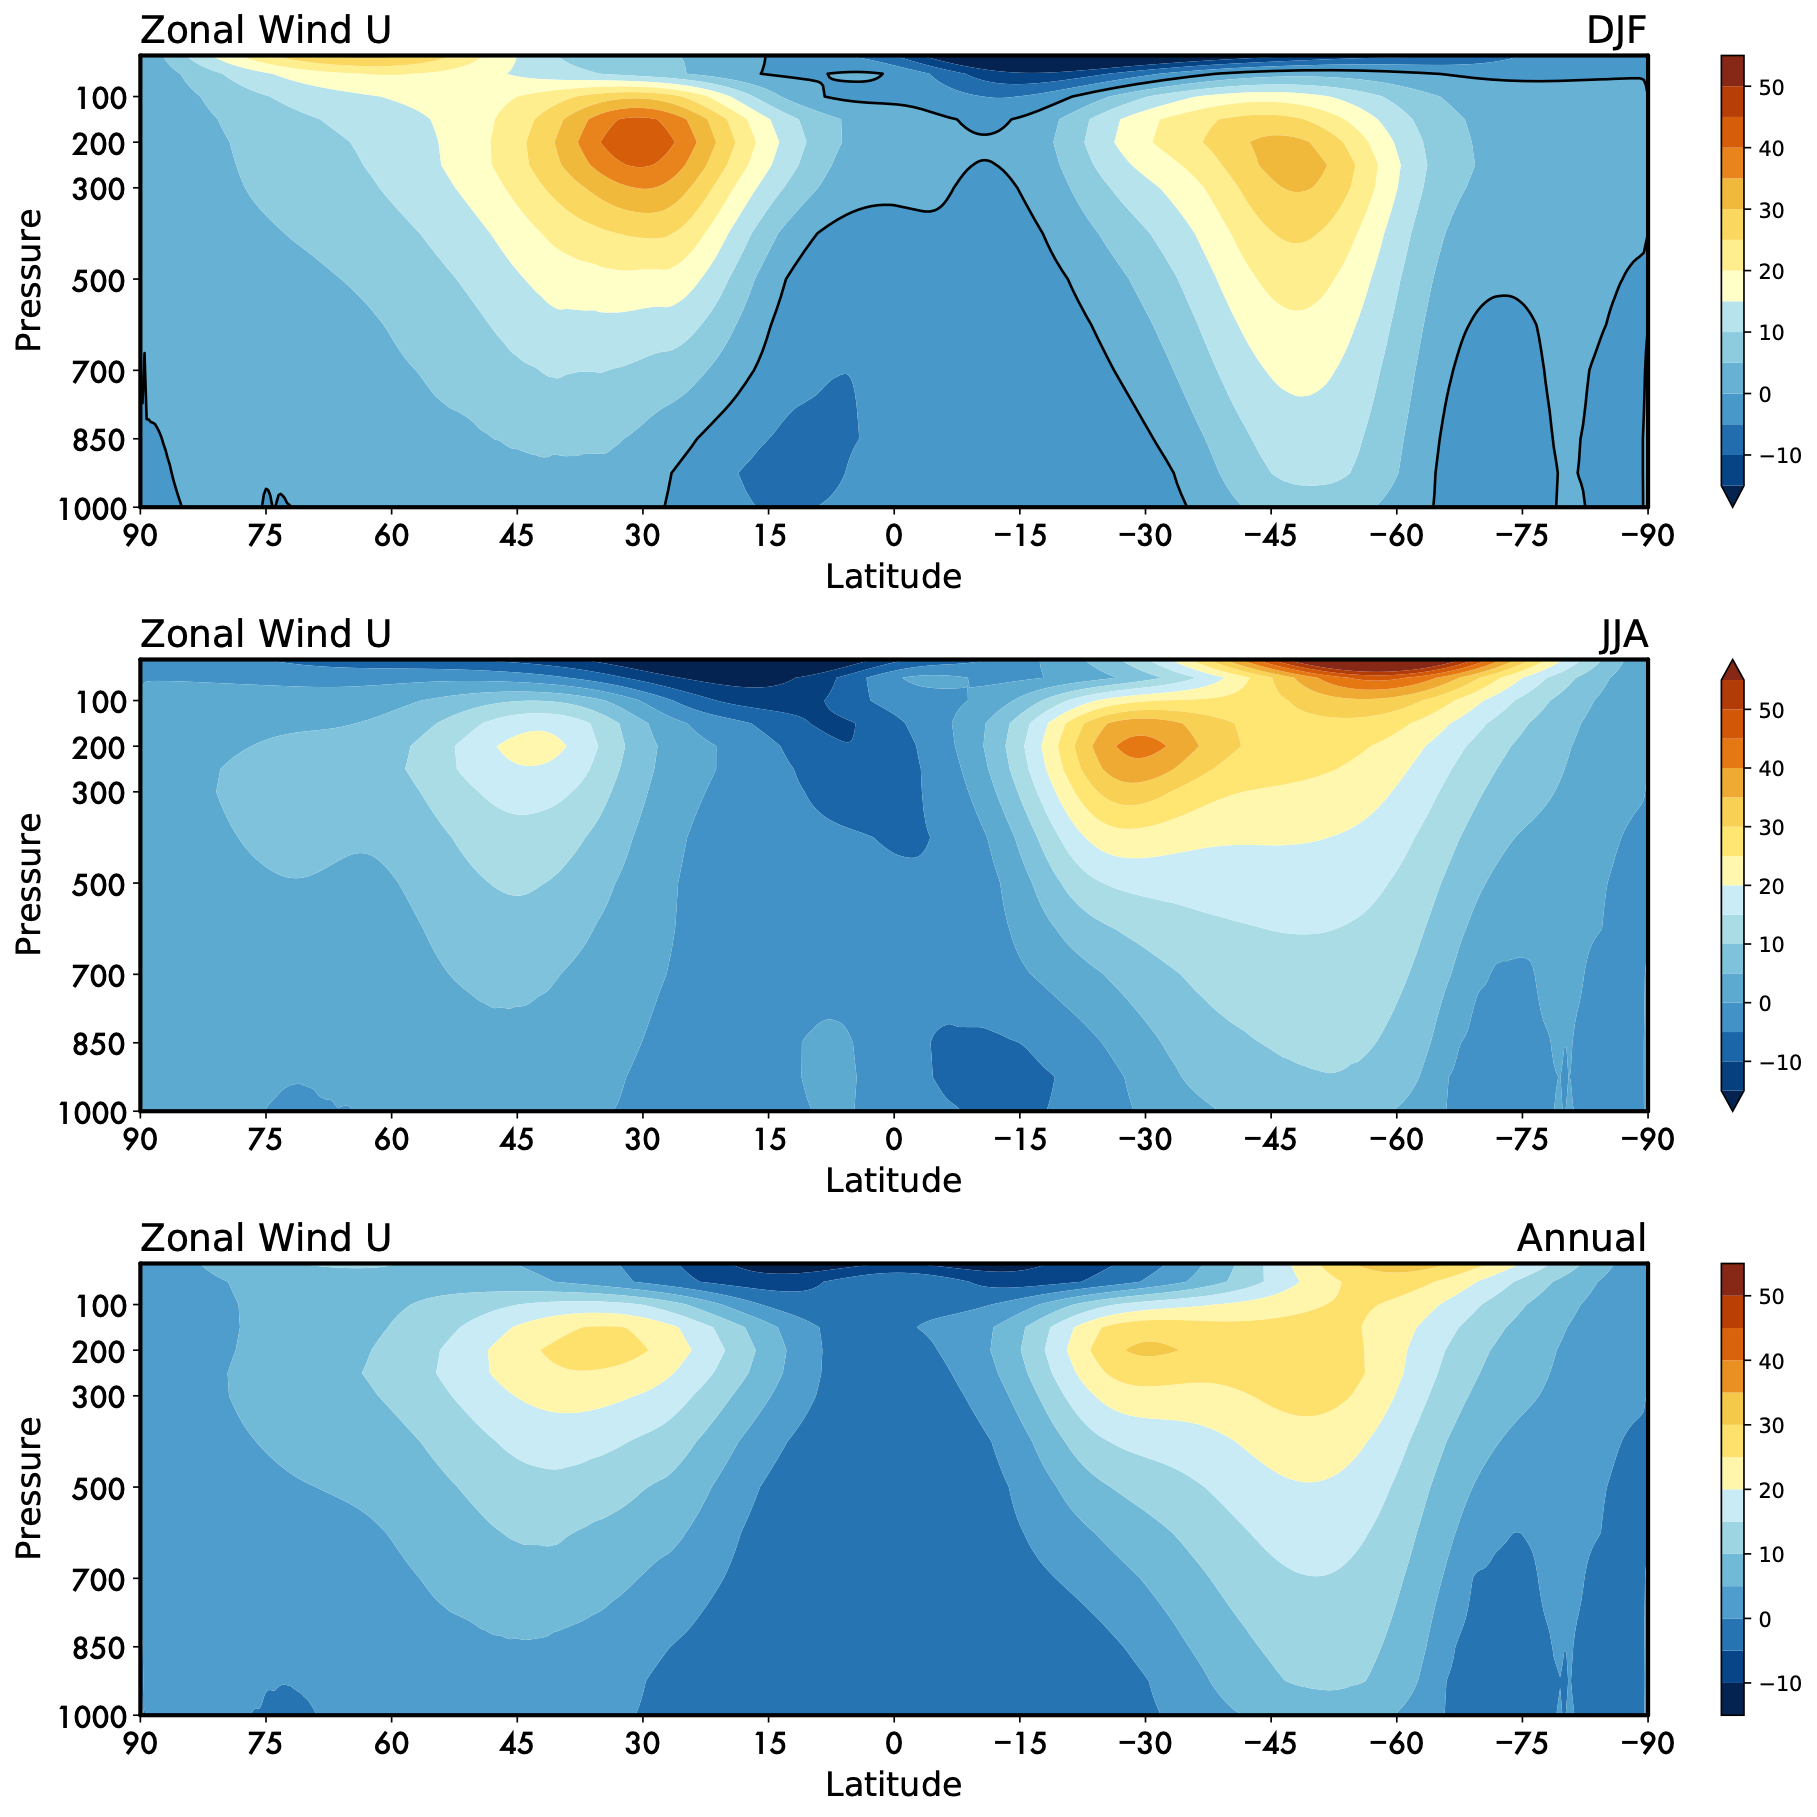
\includegraphics[width = .7 \textwidth]{figs/GD/Uzonal.png}
\caption{}\label{}
\end{figure}

The zonally averaged meridional circulation is shown in
Fig.(\texttt{fig:52}). It is possible to see the low level convergence
at the equator and high level divergence of the flow. The annual mean
show more clearly the direct circulation that is located between the
tropics. Note that the point of convergence, the InterTropical
Convergence Zone  ITCZ, though is generally following the seasonal
cycle of the sun is asymmetric with respect the equator, oscillating
between \(15N\) and \(5S\).

\begin{figure}
\centering
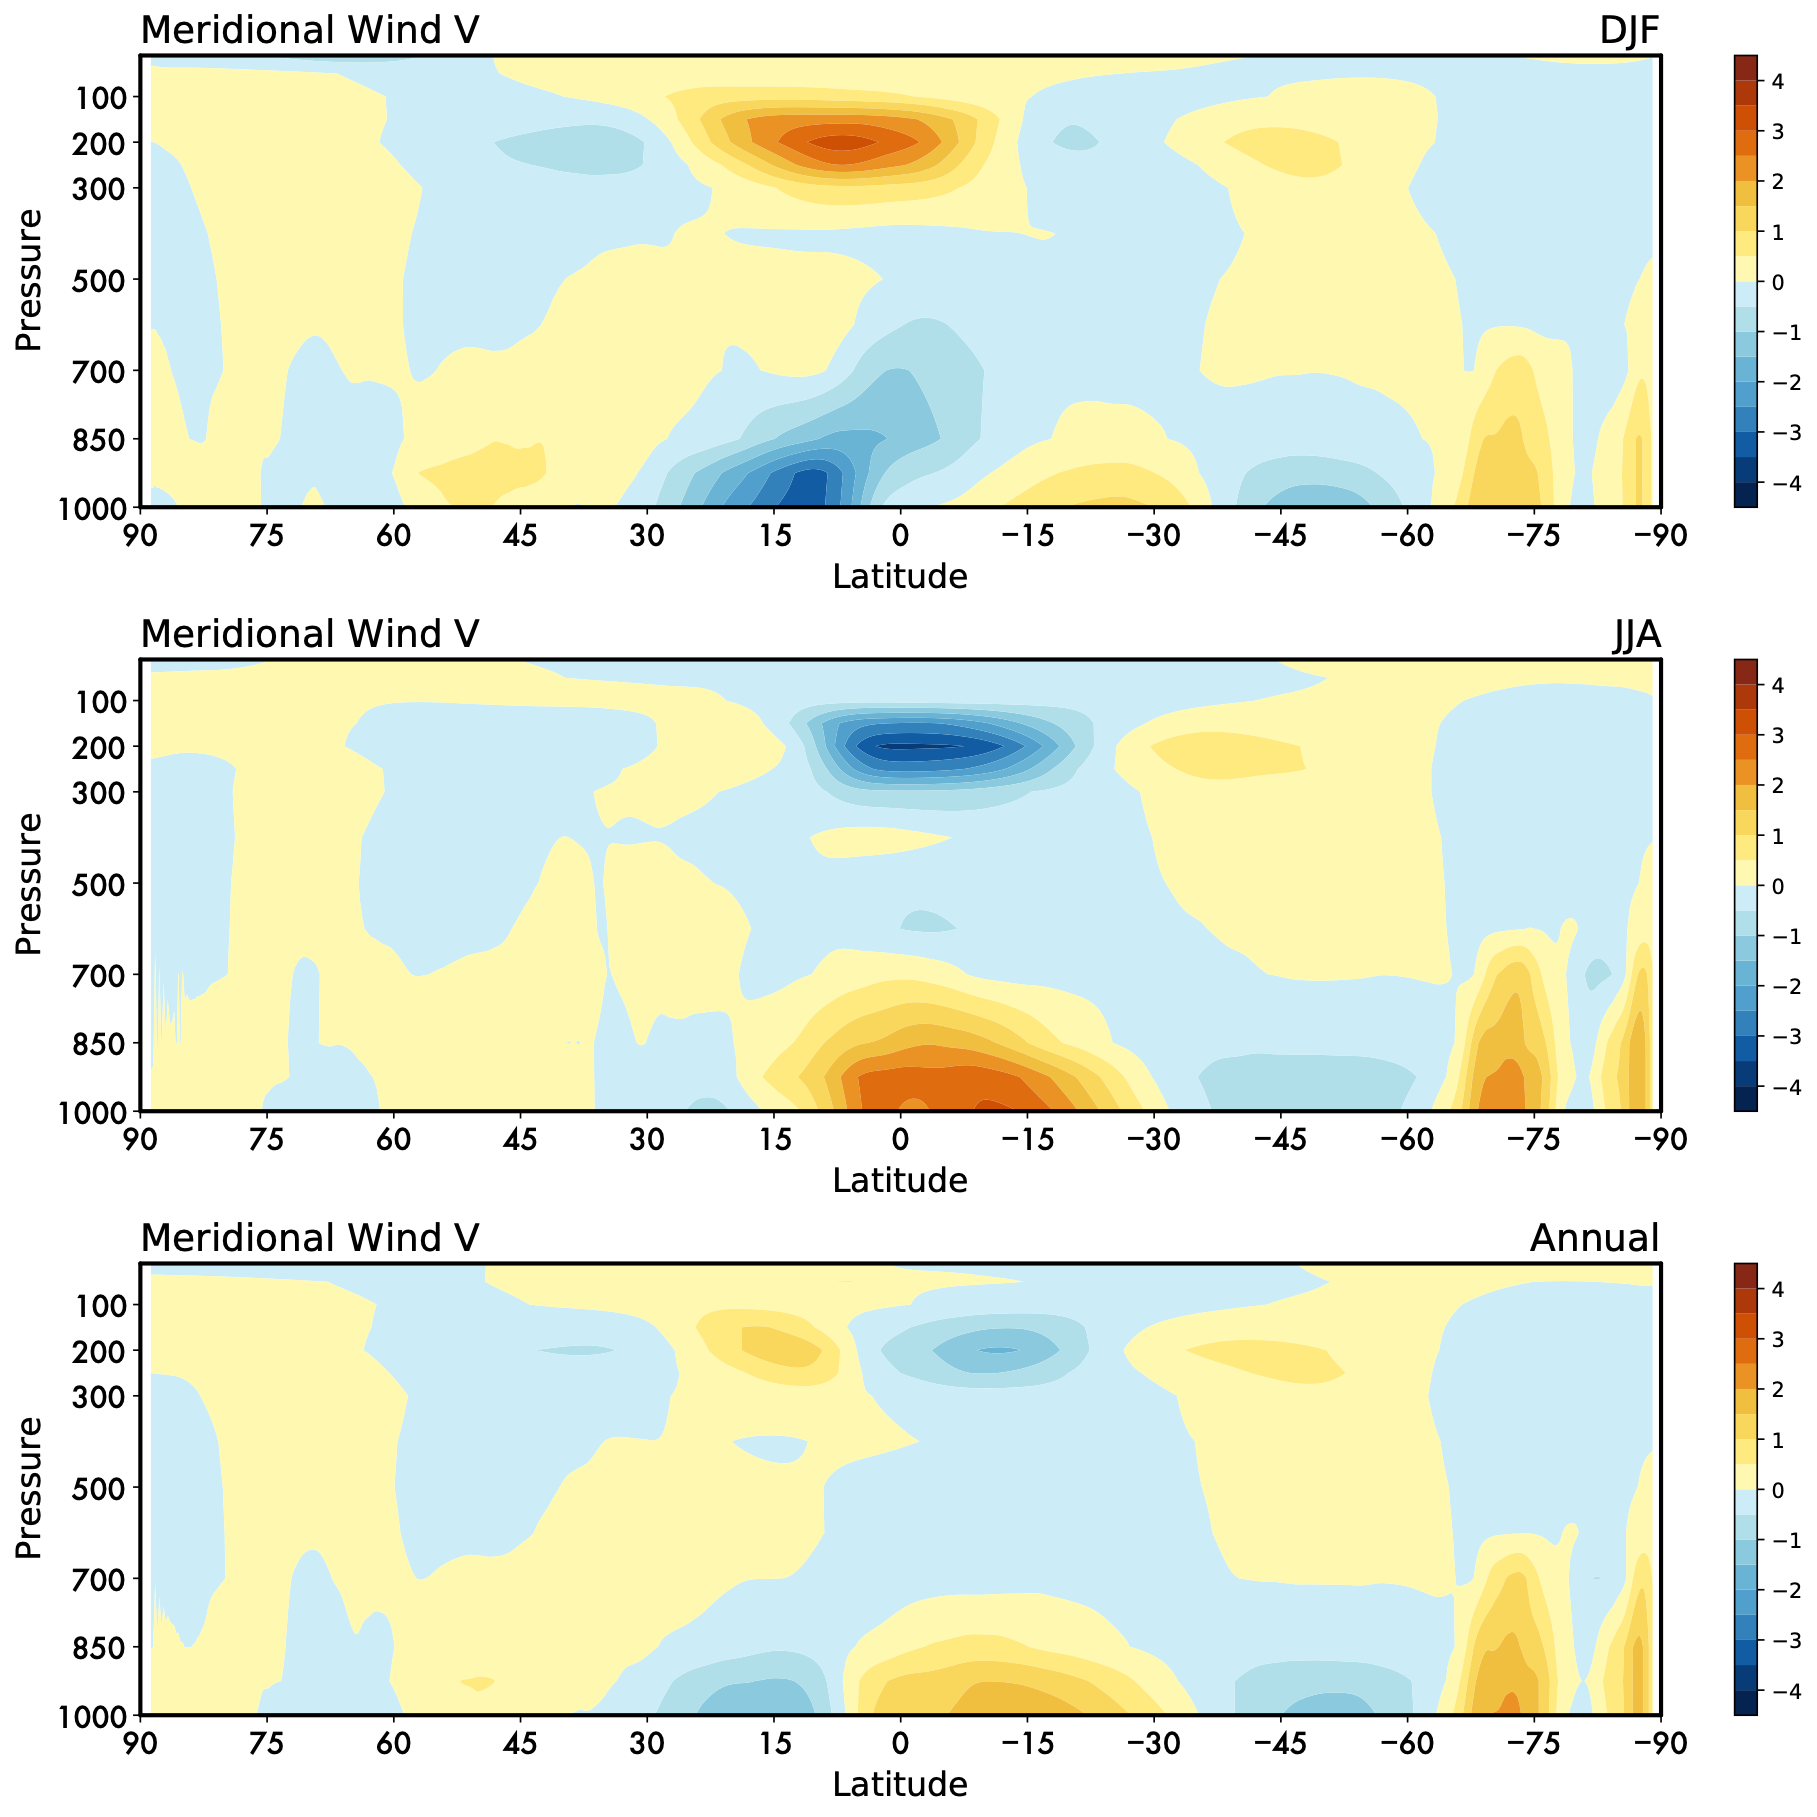
\includegraphics[width = .7 \textwidth]{figs/GD/Vzonal.png}
\caption{}\label{}
\end{figure}

The thermal structure is shown in Fig. \texttt{fig:53}. As a consequence
of the radiation balance the temperature is decreasing with latitude.
The equatorial area is receiving excess radiation with respect to the
the polar region. The hydrostatic balance is shown in the decreasing
temperature with height, but the lapse rate is less than adiabatic,
indicating the average stable nature of the atmosphere. There is a
strong latitudinal gradient in temperature, but the gradient is
decreasing with altitude and is actually reversing sign in the upper
atmosphere and stratosphere.

This is caused by the radiation absorption by ozone and other components
in the lower stratosphere. The change of sign of the temperature
meridional gradient Fig. \texttt{fig:531} is also consistent with the
structure of the zonal wind, with positive shear in the troposphere and
negative shear above it, consistent with the thermal wind balance.

\begin{figure}
\centering
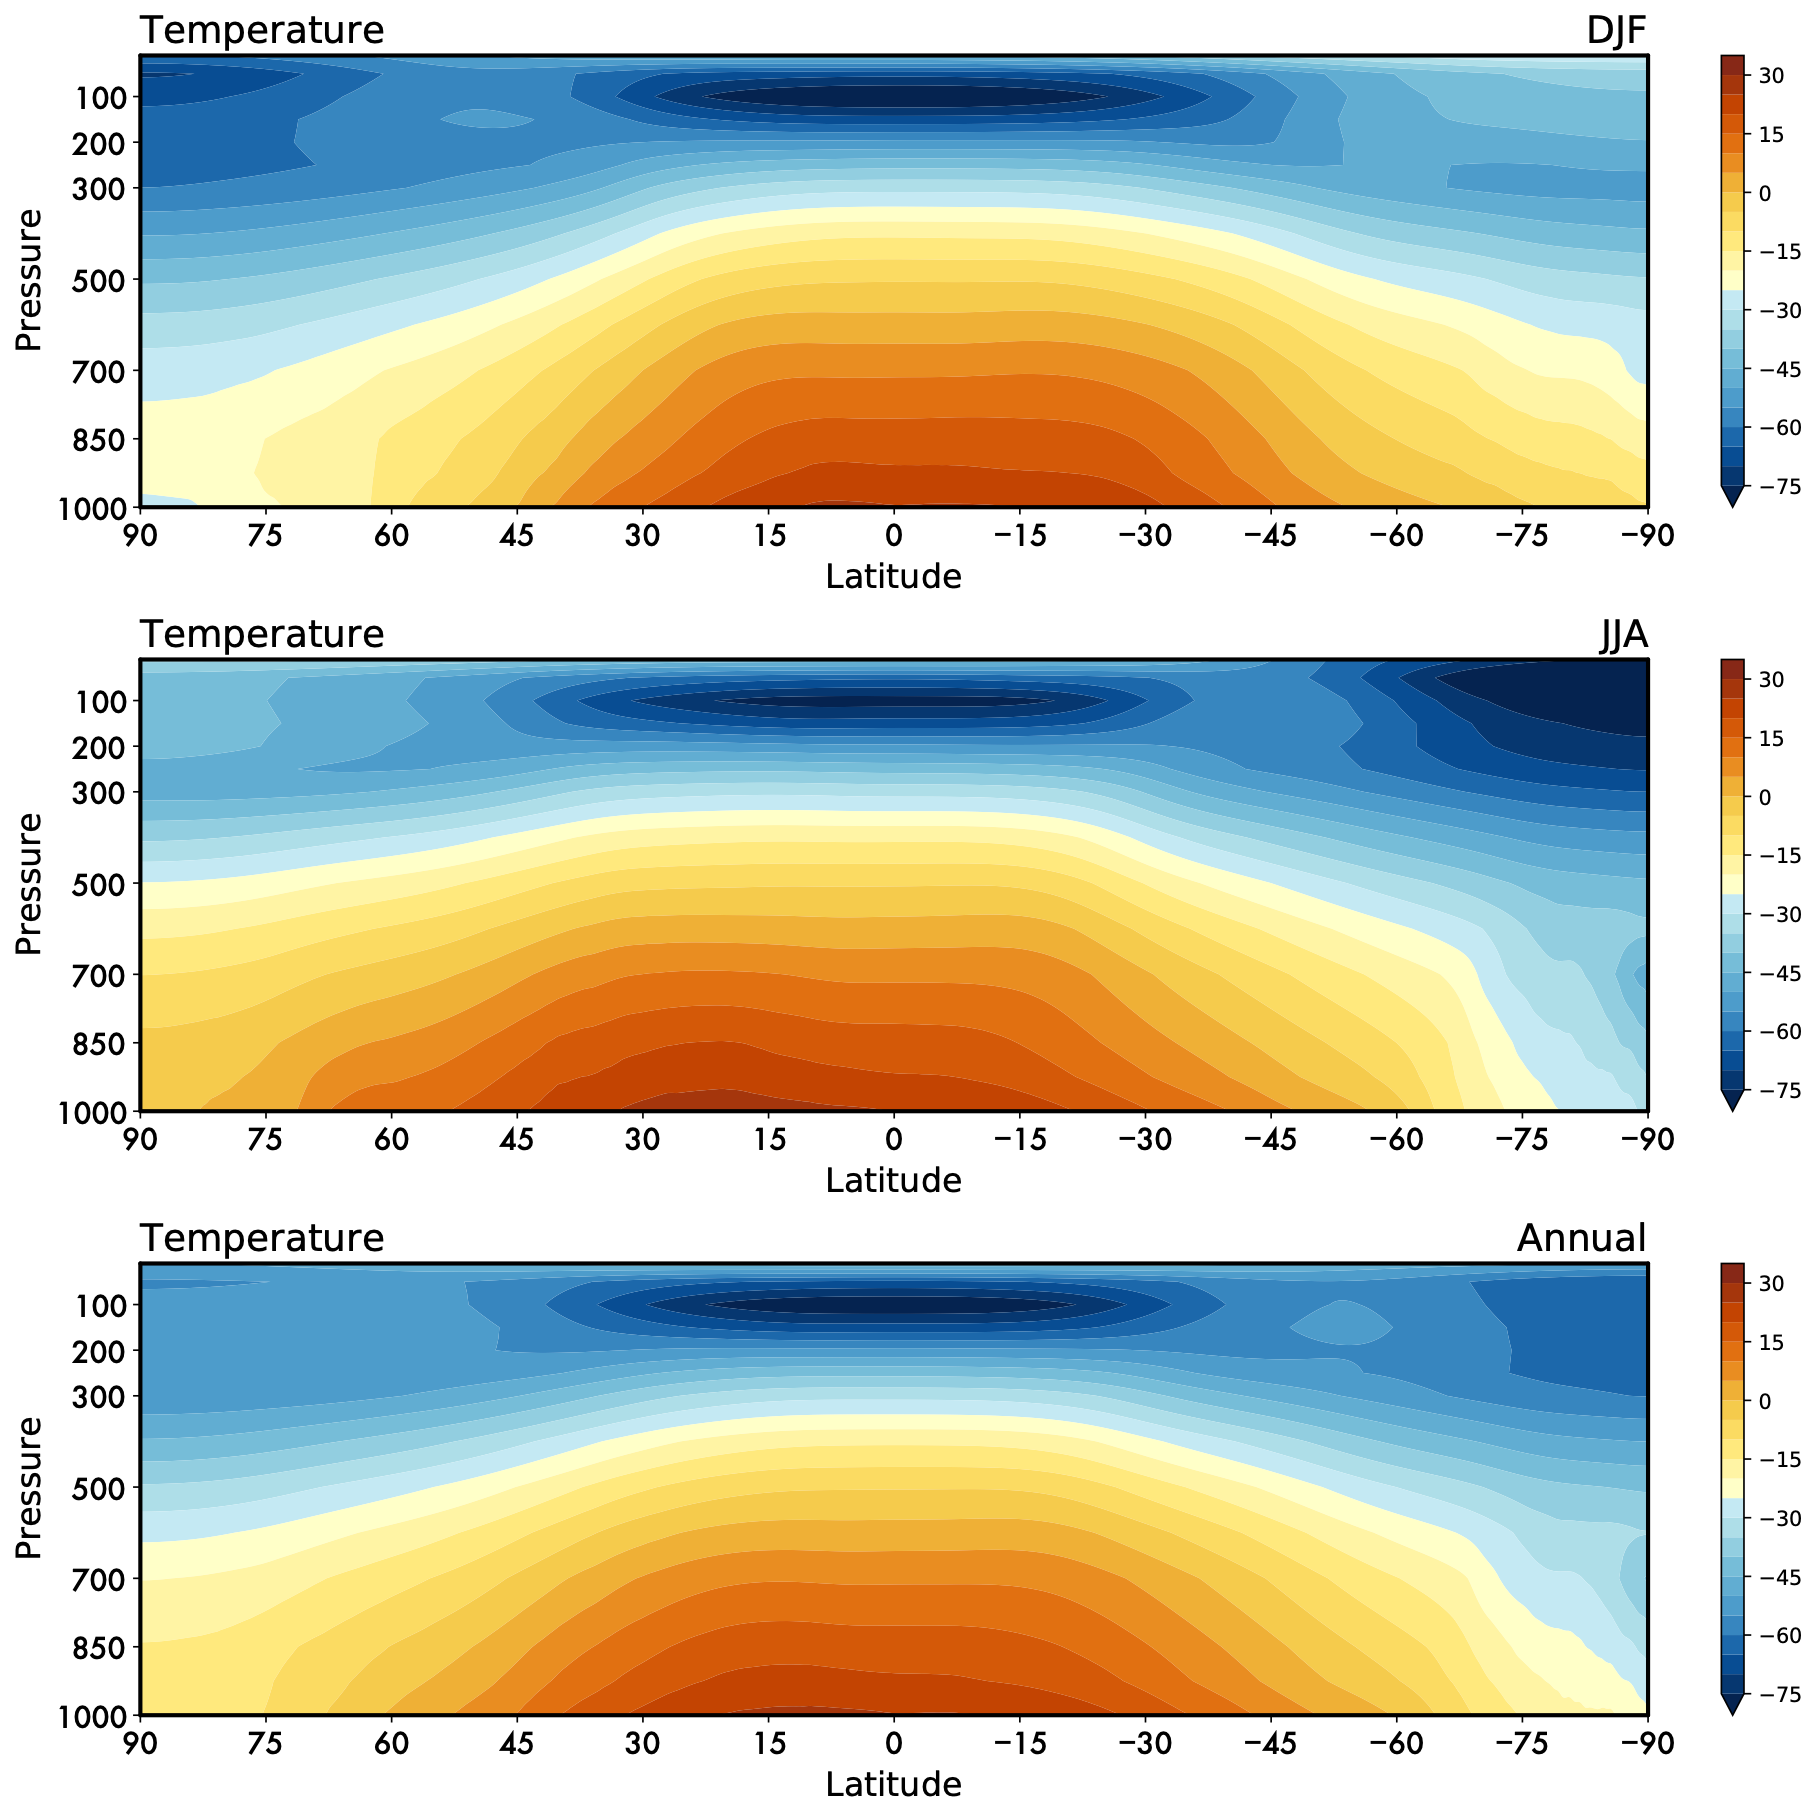
\includegraphics[width = .7 \textwidth]{figs/GD/Tzonal.png}
\caption{}\label{}
\end{figure}

\begin{figure}
\centering
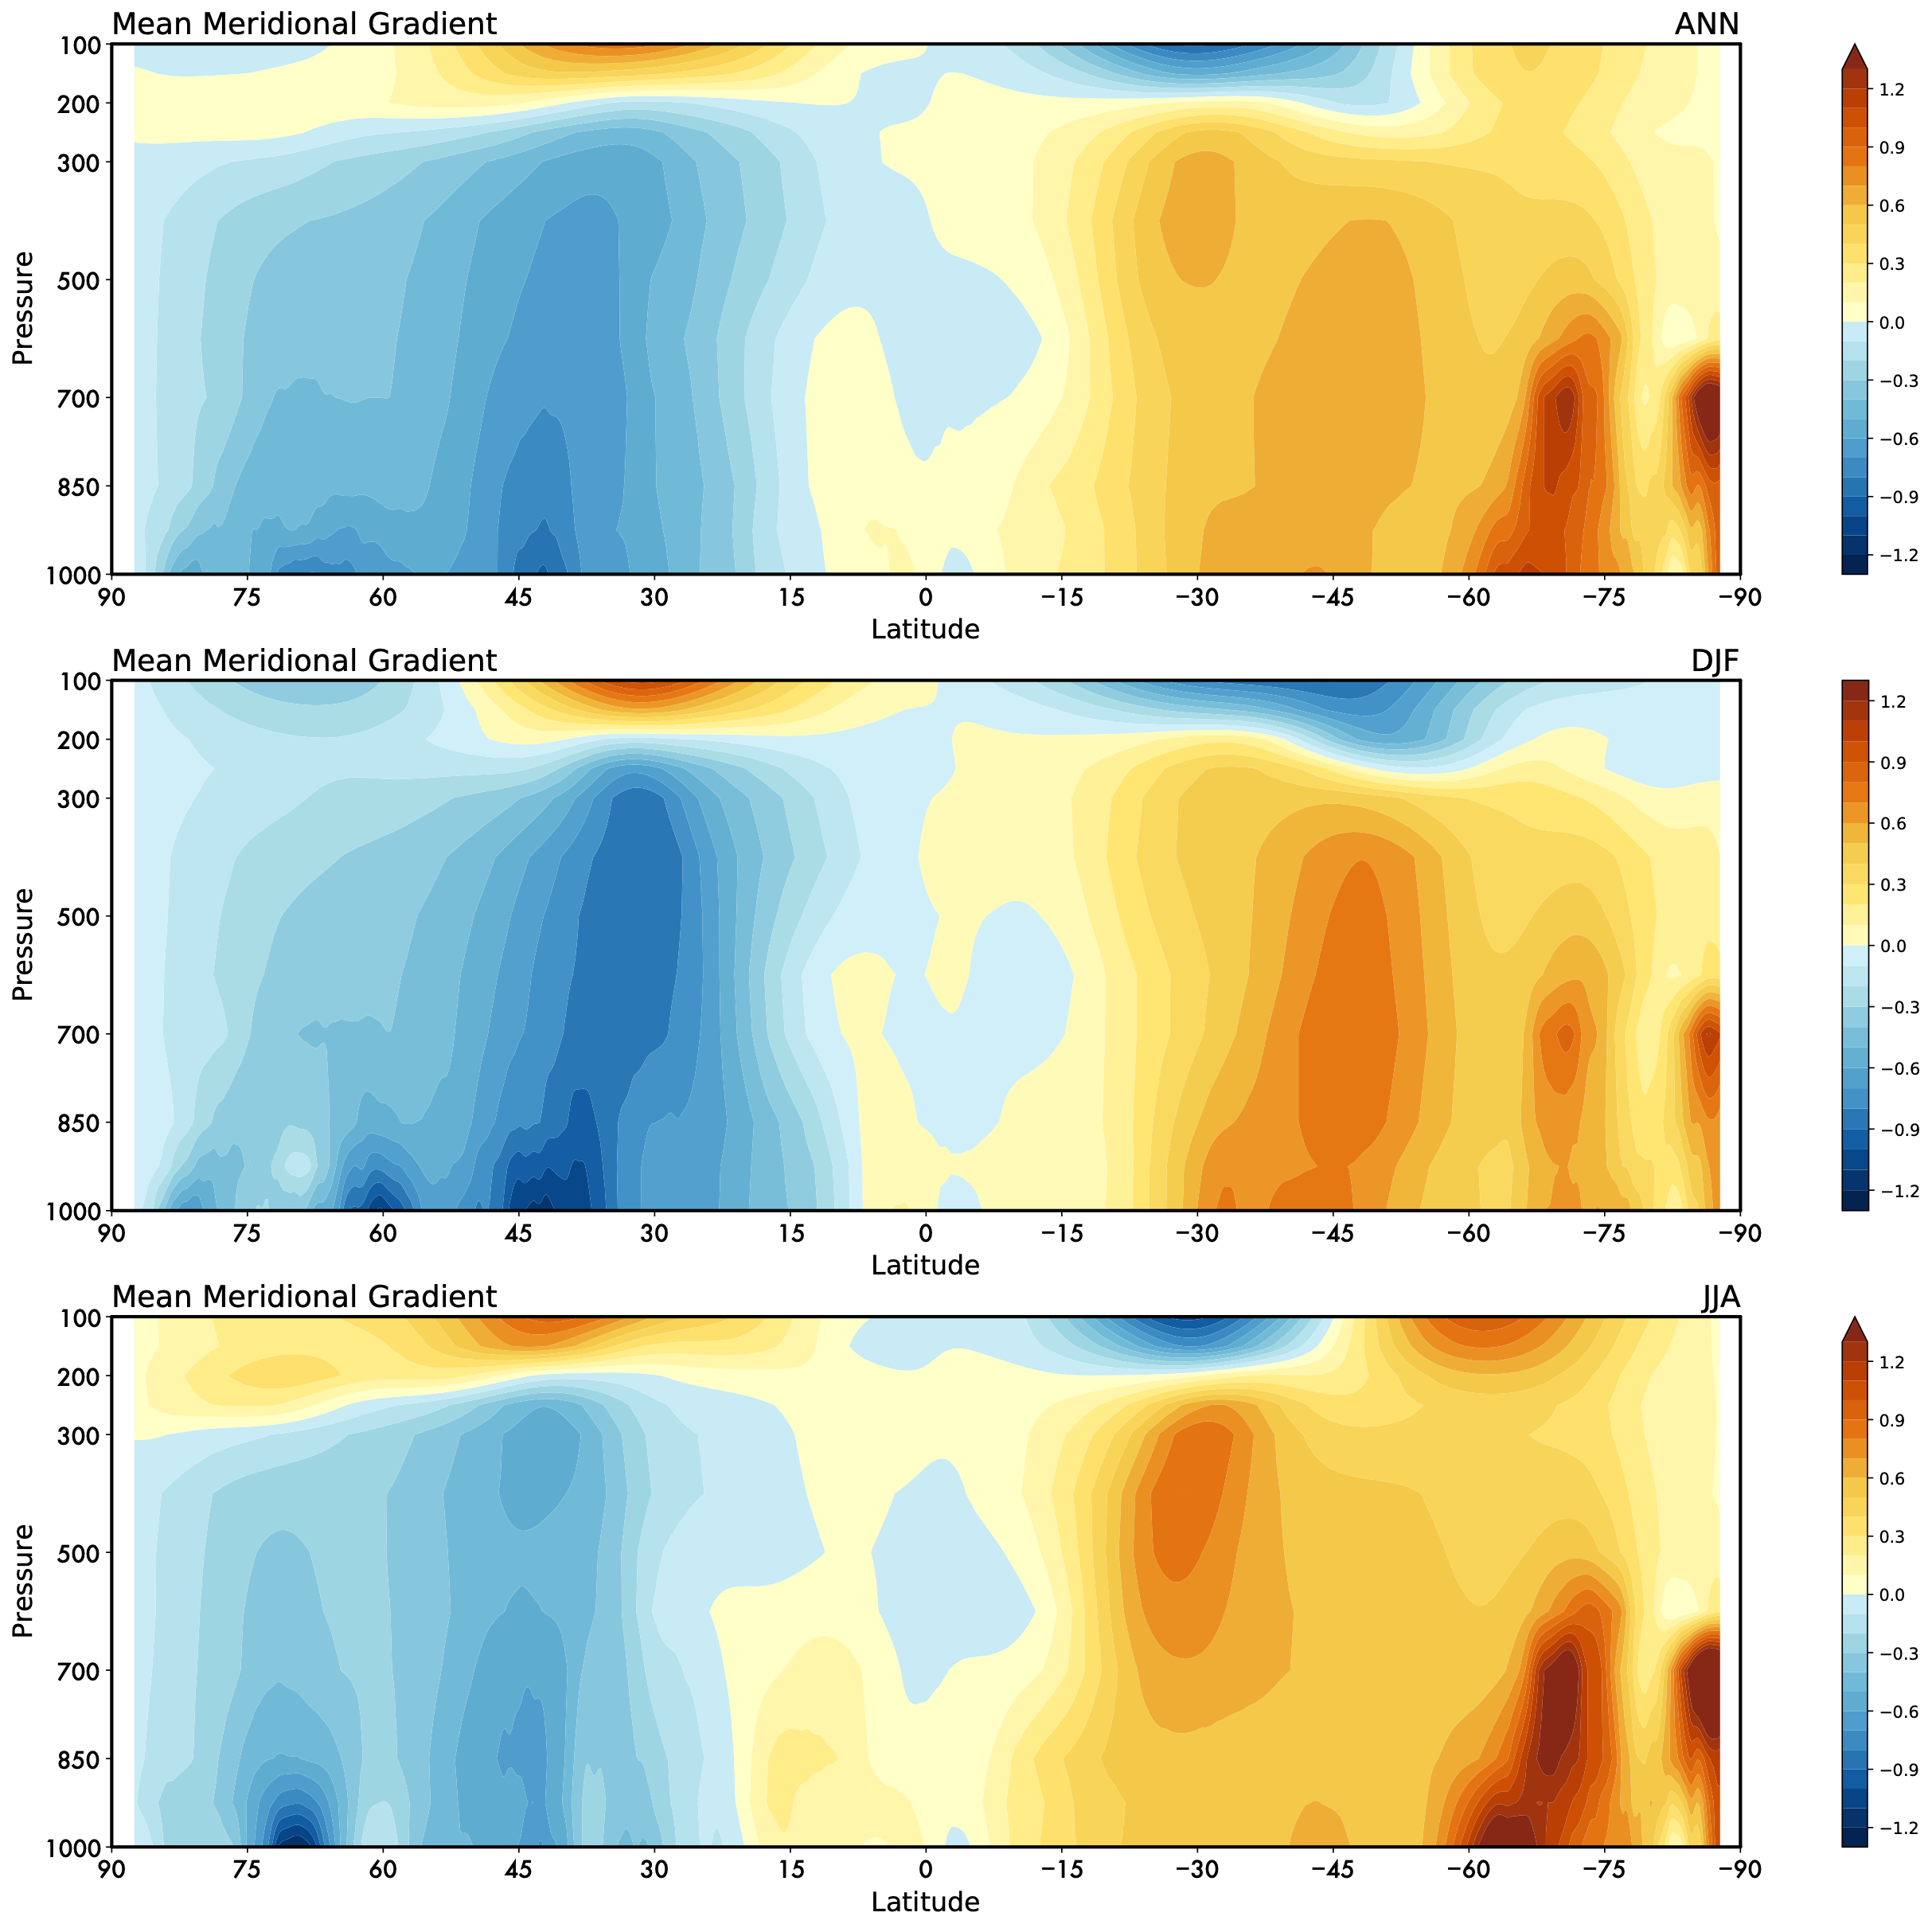
\includegraphics[width = .7 \textwidth]{figs/GD/Tgradient.png}
\caption{}\label{}
\end{figure}

The structure of the distribution of water vapor in the atmosphere is
shown in Fig. \texttt{fig:532}. The water vapor is shown as the
\emph{specific humidity} that is mass of water vapour in a unit mass of
moist air, usually expressed as grams of vapour per kilogram of air. The
annual average (bottom) shows how the water vapor is strongly confined
to the lower levels and to the equatorial zone. The atmosphere is very
dry as the altitude increases. This is a direct consequence of the
strong dependence on temperature of the Clausius-Clayperon equation that
describes how the saturation water vapor pressure changes with
temperature. At the equator, really moist air contains 12-15 grams of
water per kilogram of moist air.

The seasonal distributions (other panels in Fig. \texttt{fig:532}) show
a shift of specific humidity in latitude roughly following the seasonal
cycle of the sun. The surface maximum is located around 5S in DJF and
then shifts to around 10N in JJA. The Winter hemisphere in both seasons
is definitely more moist at the surface than the Summer, but values are
smaller than the equatorial zone, reaching at most around 8 g/kg.

\begin{figure}
\centering
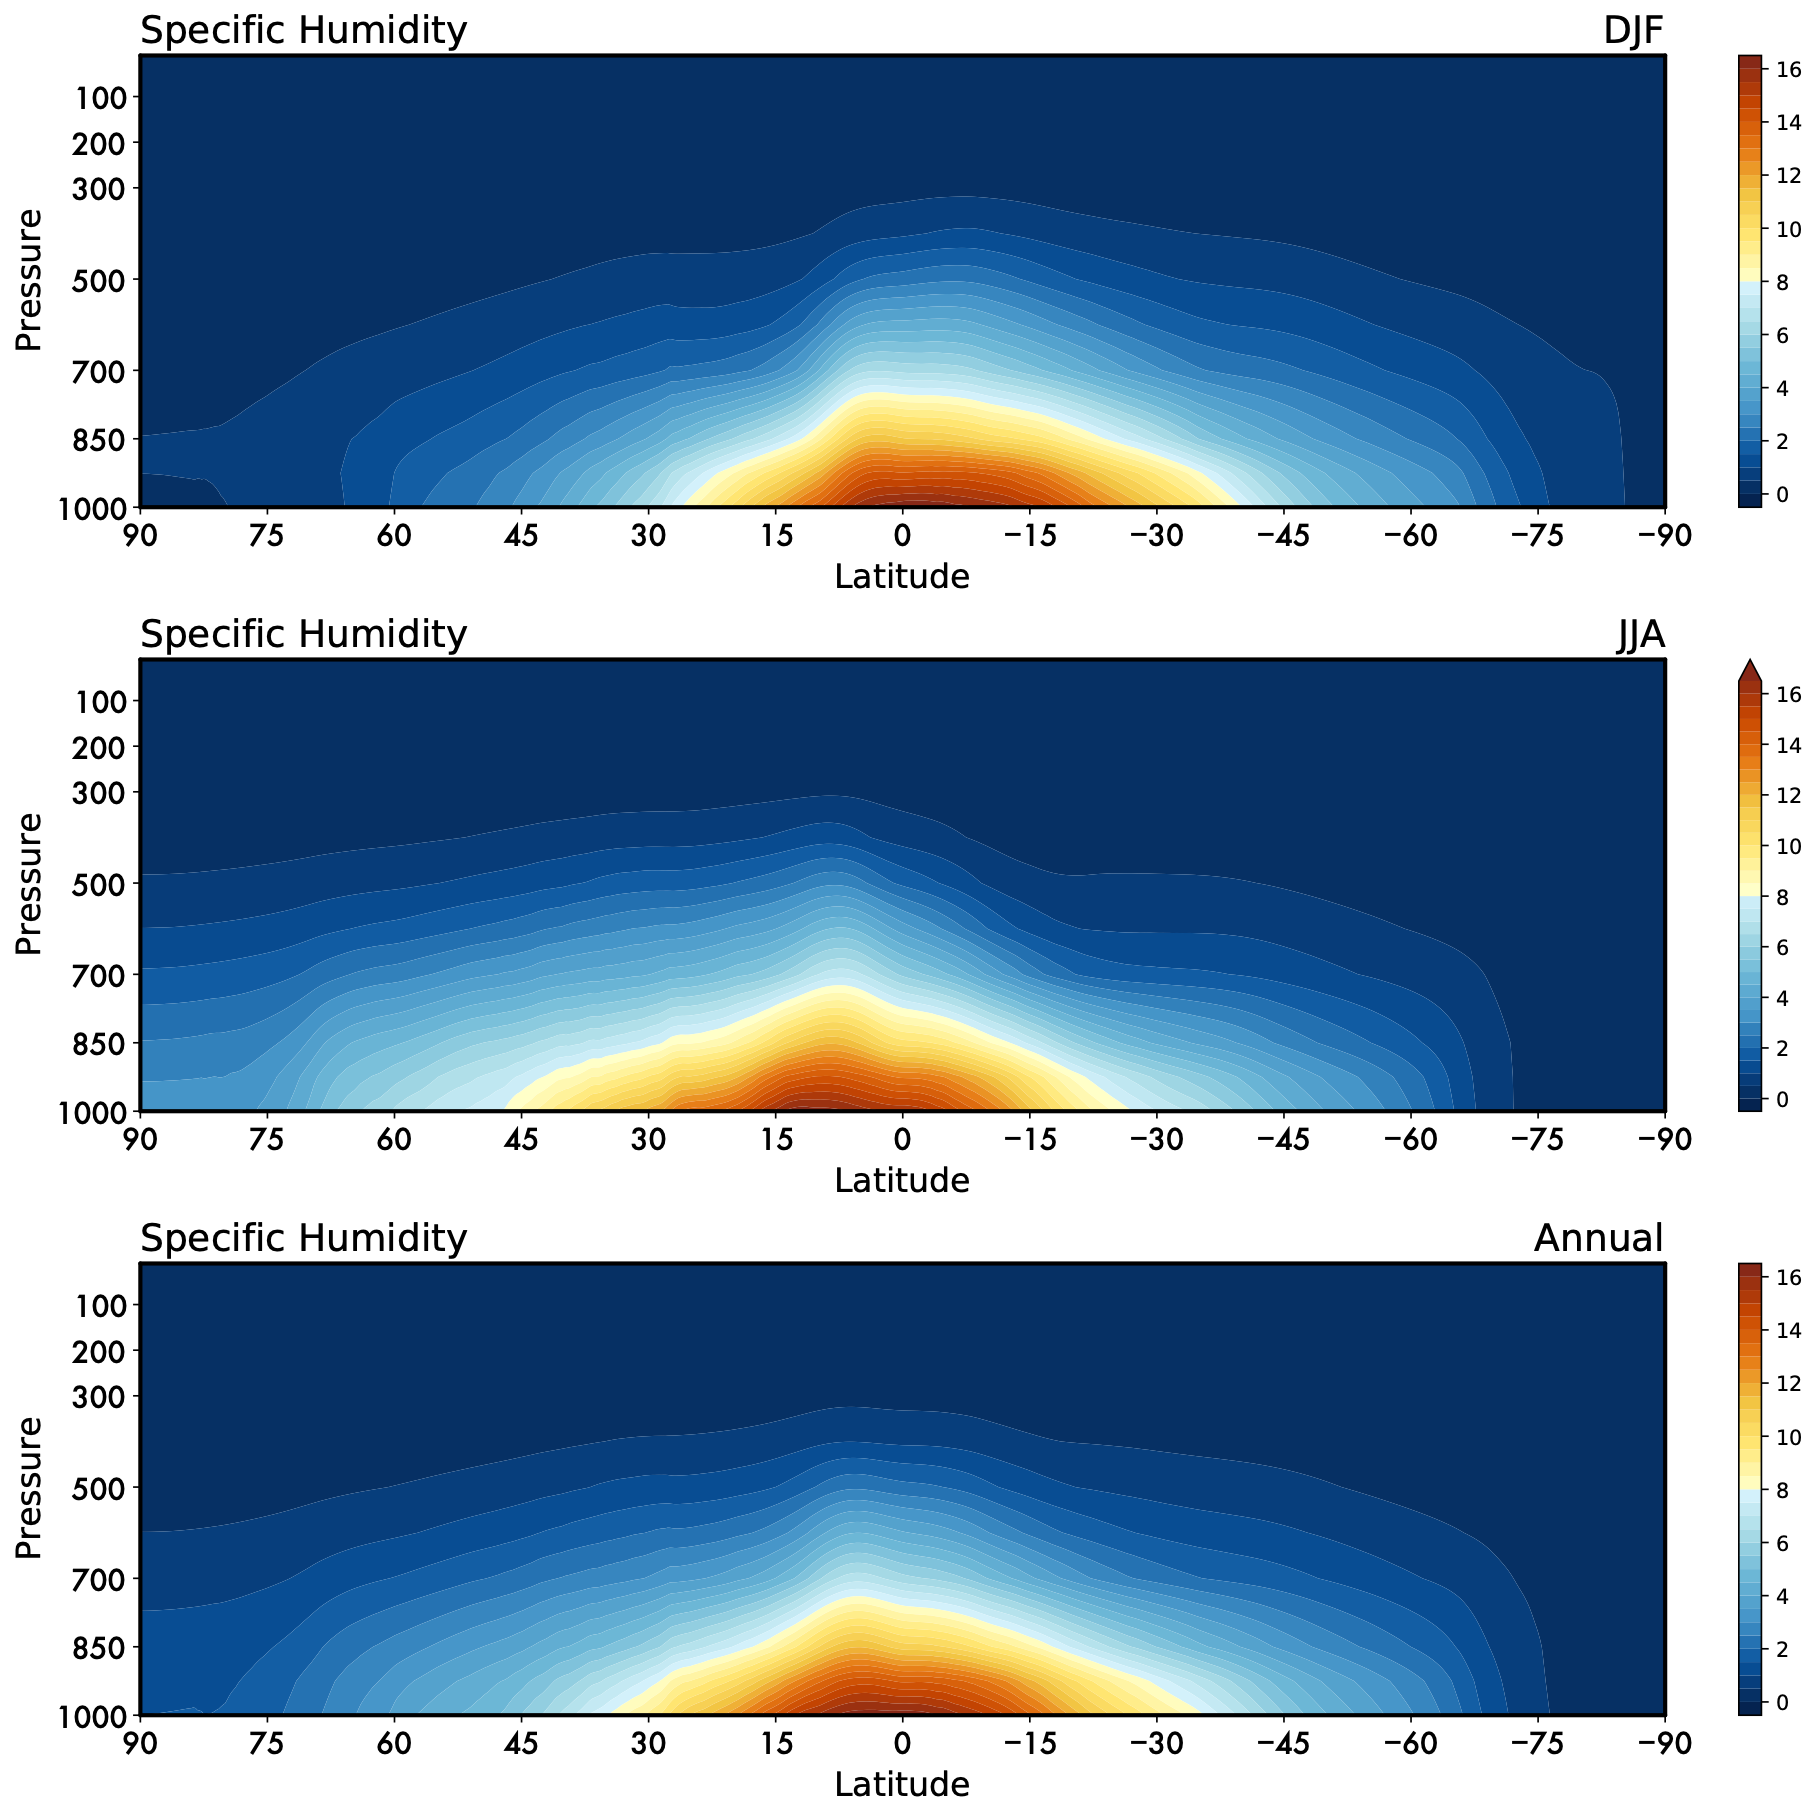
\includegraphics[width = .7 \textwidth]{figs/GD/Qzonal.png}
\caption{}\label{}
\end{figure}

. {[}fig:532{]}

\begin{figure}
\centering
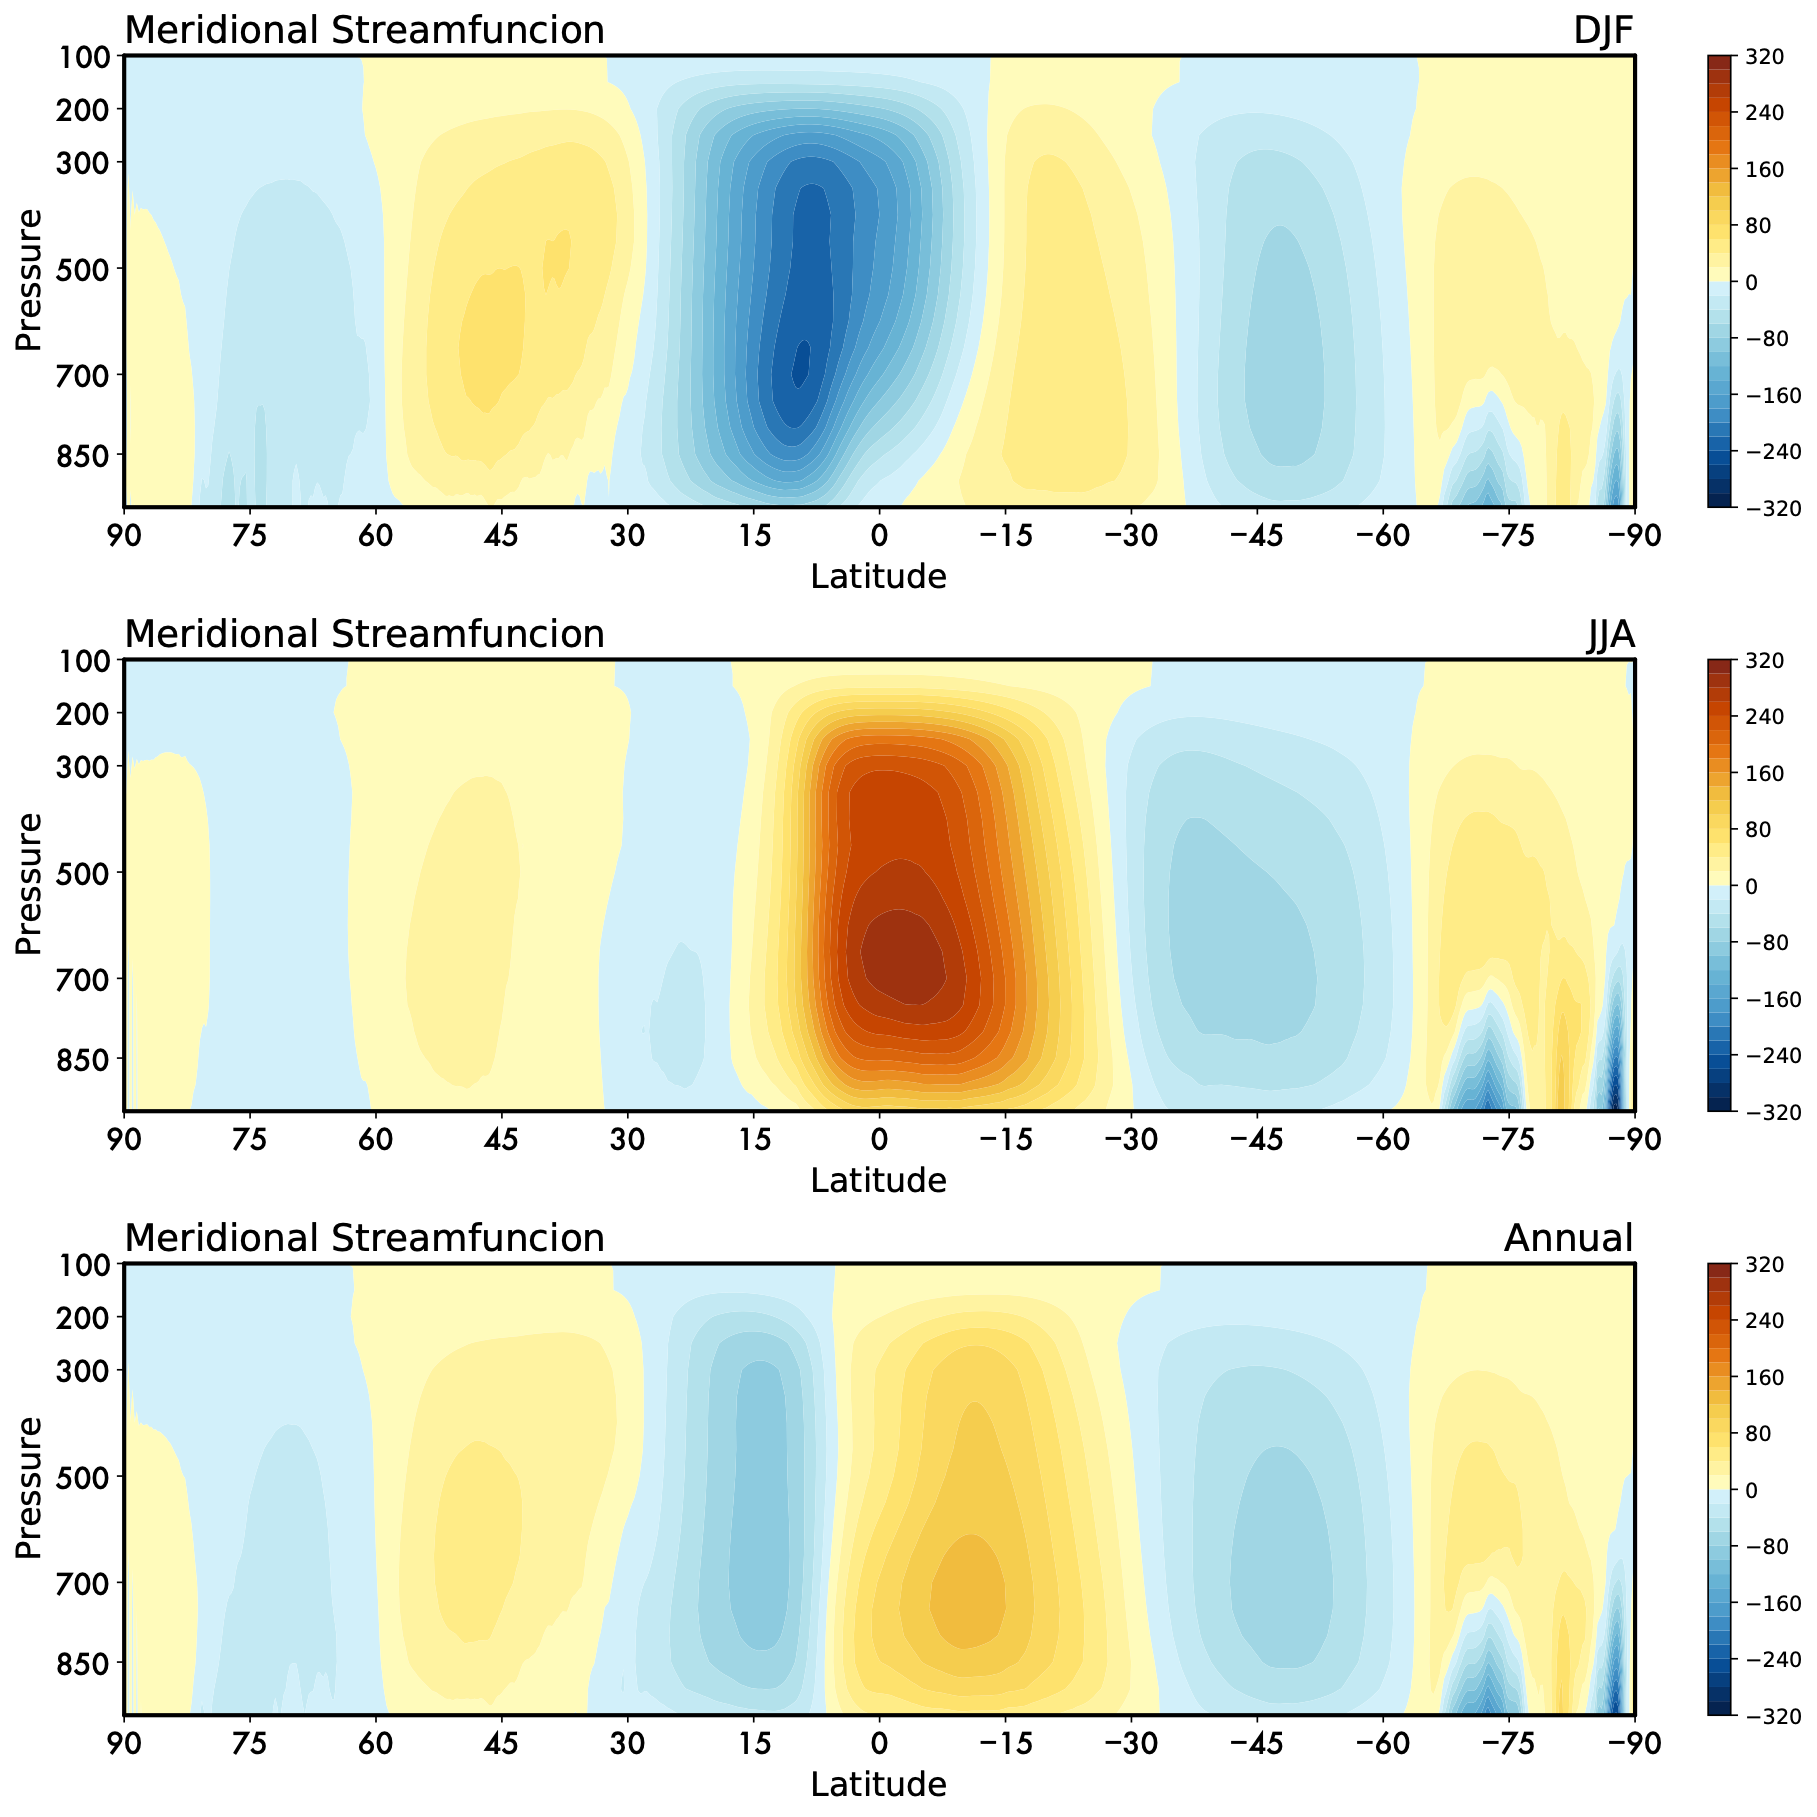
\includegraphics[width = .7 \textwidth]{figs/GD/MSzonal.png}
\caption{}\label{}
\end{figure}

\subsection{The horizontal general
circulation}\label{the-horizontal-general-circulation}

Fig. \texttt{fig:551} shows the climatological geopotential height for
DJF at 200mb. The top panel shows the full field. The geostrophic
balance implies that it can be considered as an approximate
streamfunction for the horizontal flow. The bottom panel shows the same
field with the zonal mean removed, the eddy component. It shows clearly
the large deviations from the zonally symmetric circulation located over
the east coast of continents. A more careful inspection may reveal that
they are downstream from large continental size mountain ranges, the
Rocky Mountains and the Himalayan Plateau.

\begin{figure}
\centering
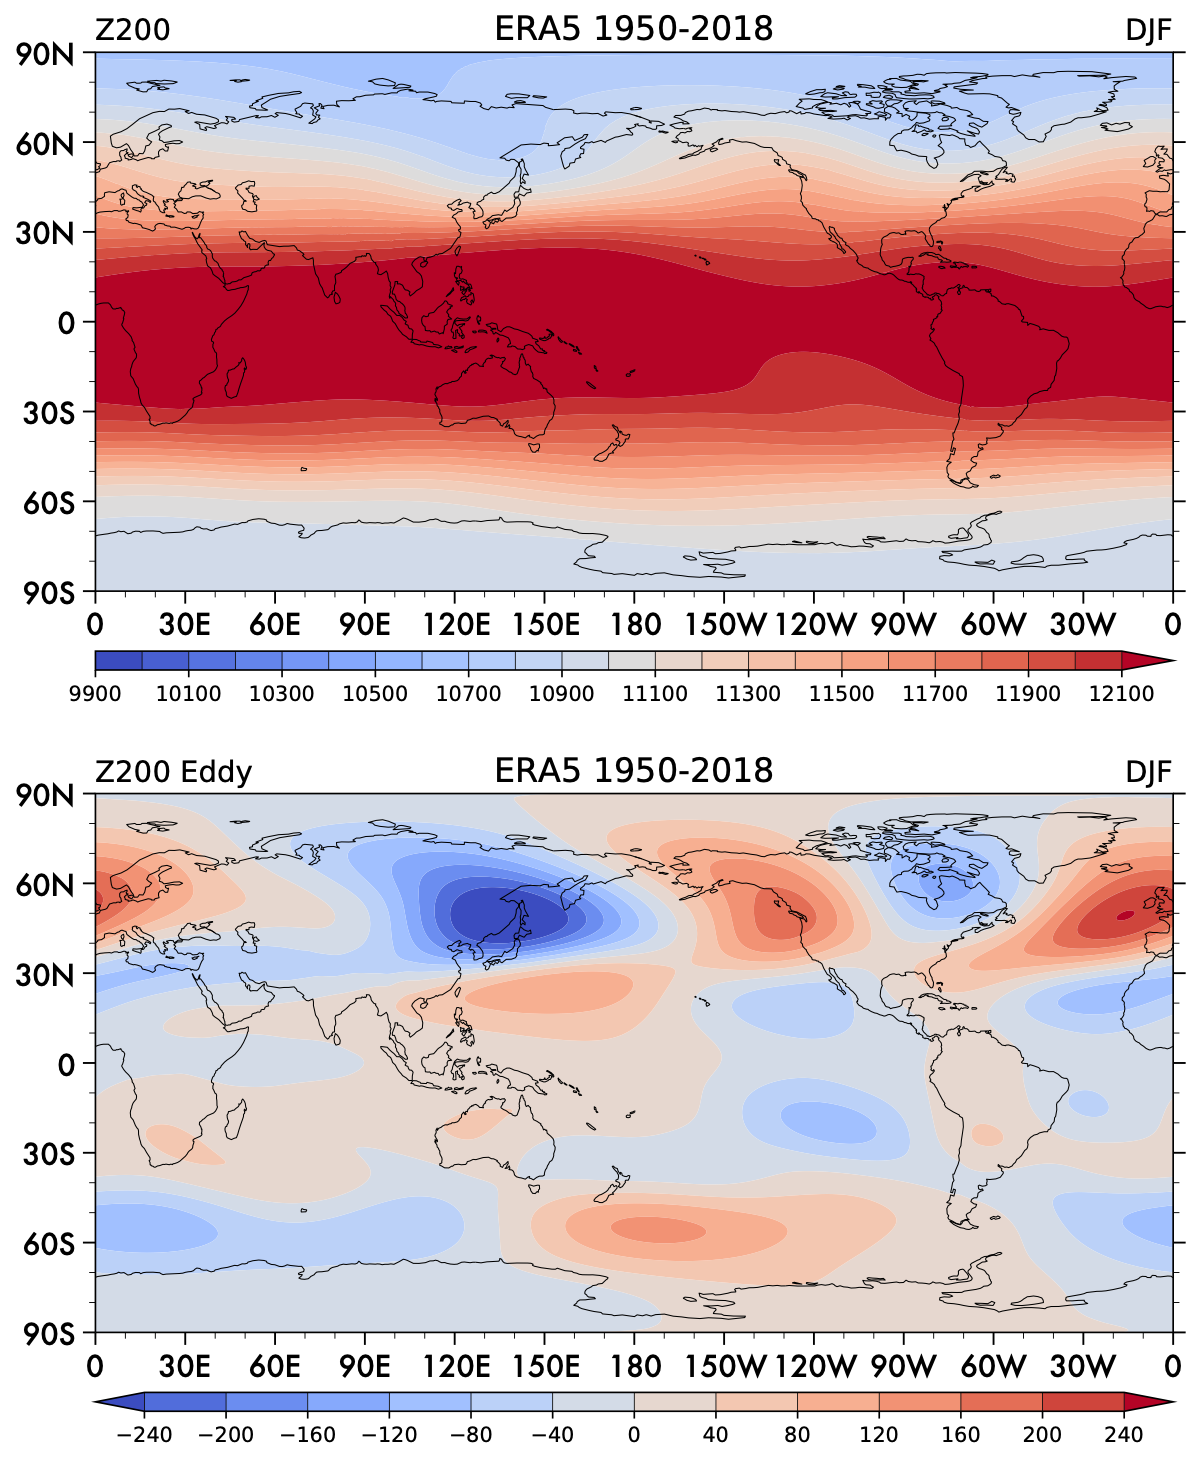
\includegraphics[width = .7 \textwidth]{figs/GD/Z200.png}
\caption{}\label{}
\end{figure}

A better insight is provided by using a special polar projection to
inspect the Geopotential field. There are several geographical
projection to represent quantity on the sphere on a map and each of them
is useful to enhance some property of the flow. The shape of the
hemispheric circumpolar vortex is for instance clearly represented in
the stereo projection of Fig. \texttt{fig:552}. it is possbile to see
the curvature of the flow downstream of the Rocky Mountains and the
Himalayas and the typical shape of the Winter climatological pattern of
the high altitude atmospheric geopotential.

\begin{figure}
\centering
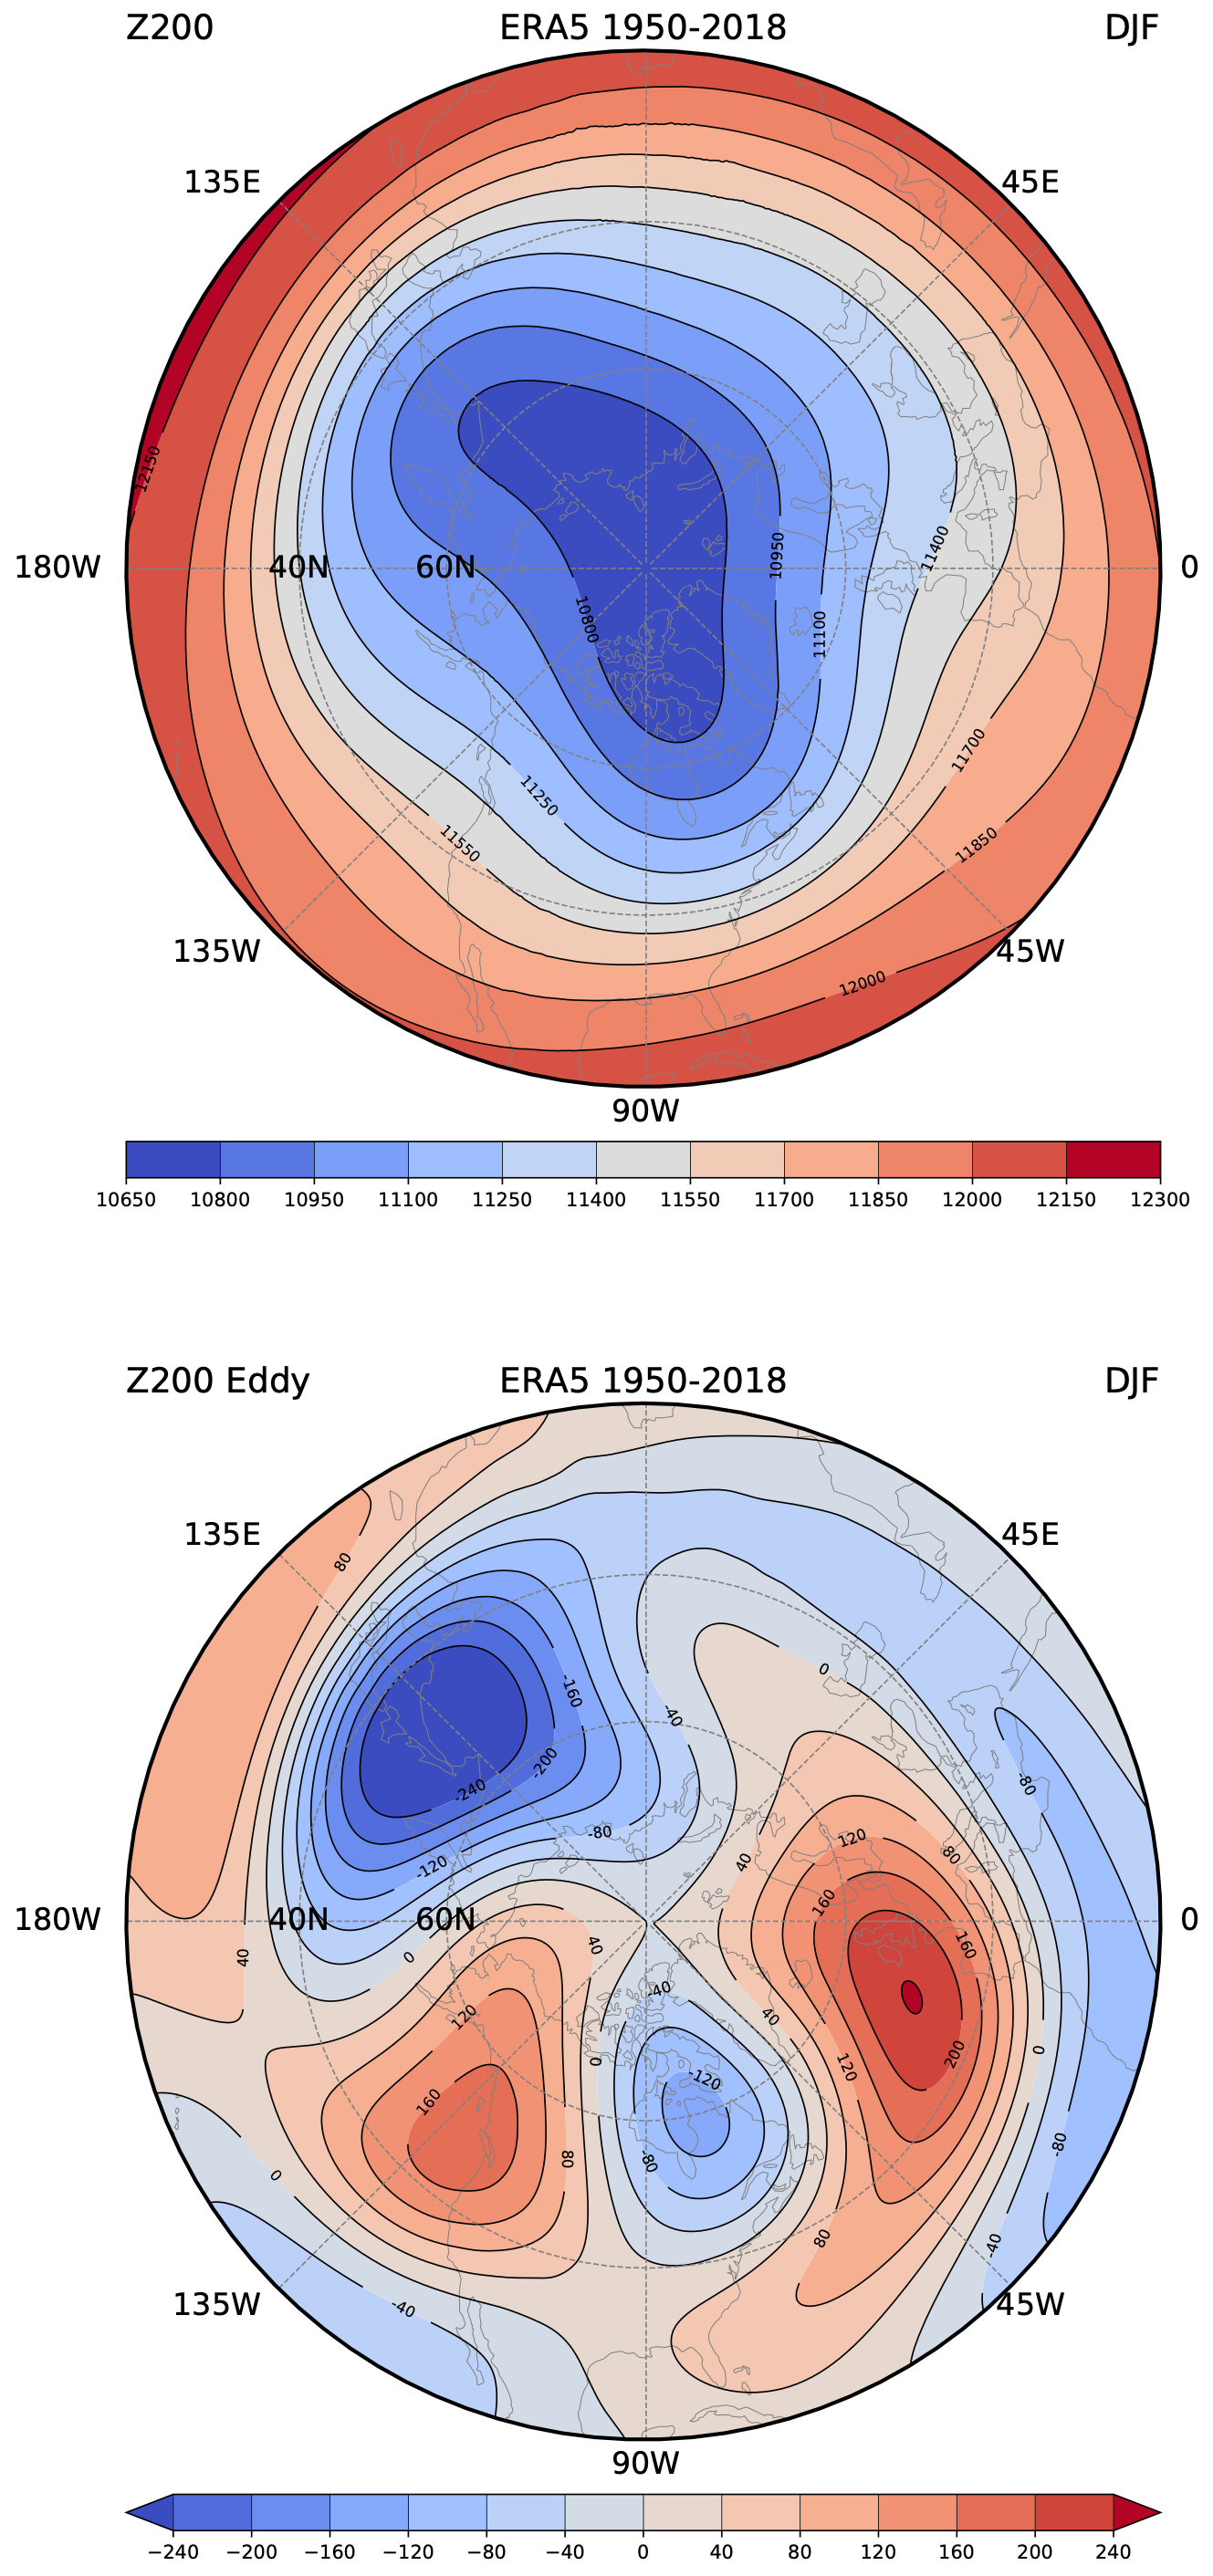
\includegraphics[width = .7 \textwidth]{figs/GD/Z200NH.png}
\caption{}\label{}
\end{figure}

\subsubsection{The horizontal wind}\label{the-horizontal-wind}

The geopotential is a good approximation to the streamfunction in the
mid-latitudes where the geostrophic balance controls tightly the
dynamical balance, but it gives usa poor ideas of the wind circulation
in the low latitudes. In this case is better to look at the wind
directly. Fig. \texttt{fig:56} shows the zonal wind at 200mb for the
calendar Winter (DJF) and Summer (JJA). We can see clearly the westerly
jet streams in the winter of both hemispheres. The jets are concentrated
on the east coast of both large continental land masses.

The Asian jet is the most intense, reaching at its core a velocity in
excess of 70 m/s. In comparison, the North American jet is weaker and
smaller in longitudinal extent. The winter jet in the Southern
Hemisphere is also well formed, but at this level is not at the same
amplitude of the northern hemisphere jets. Summer westerly jets are also
present in both summer hemisphere, but much weaker.

The tropical region instead is characterised by easterly jets, most
prominent over the maritime continent and the equatorial South America.
In Summer the Easterly circulation over the Indian Ocean is very
intense. The longitudinal gradient of the wind implies areas of
divergent flow over South America and the Indonesian region.

The meridional wind in winter (DJF) (Fig. \texttt{fig:57}) shows the
alternating patterns of positive and negative (poleward and equatorward)
that are consistent with the eddy pattern of the geopotential. Large
deviations from the zonal mean occur over the Pacific-North American
sector and over Far East Asia. In the calendar Summer (JJA) the winds
are weaker and they reach a somewhat large amplitude only over the
southern hemisphere.

Close to the surface (Fig. \texttt{fig:55}) the zonal wind is in general
weaker over land, but stronger over the ocean, and it is clearly
westerly in the mid latitudes, whereas easterlies dominates the
subtropical zone, with the notable exception of the Indonesian Region,
also called the Maritime Continent, where is westerly. The combination
of Easterlies and Westerlies in the equatorial Pacific point to a near
surface convergence area somewhere in the Central Pacific Ocean.

In JJA the zonal wind shows the seasonal cycle and it gets strength in
the winter hemisphere, retaining the general features that we have seen
for the Winter. Note instead the strong westerlies in the Indian Ocean.
This is the first evidence of the seasonal monsoonal circulation in the
Indian subcontinent. The Easterlies south of the westerlies indicates a
possible circulation over the Indian Ocean basin.

\begin{figure}
\centering
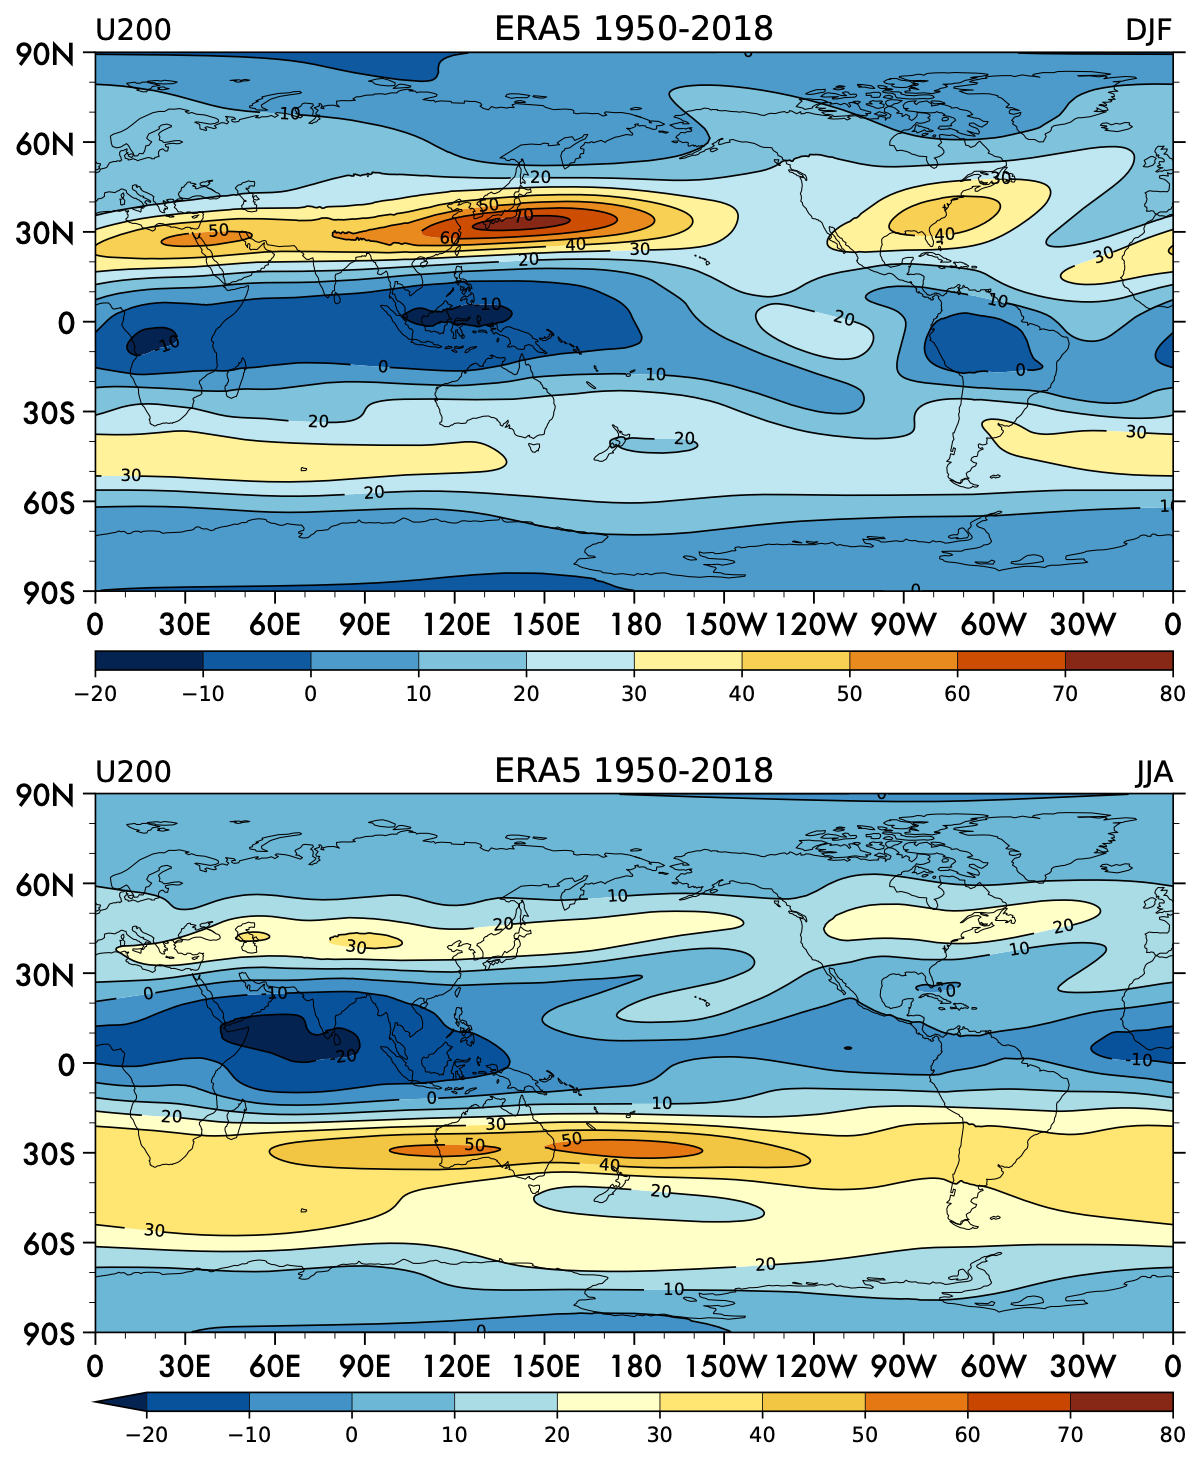
\includegraphics[width = .7 \textwidth]{figs/GD/U200.png}
\caption{}\label{}
\end{figure}

\begin{figure}
\centering
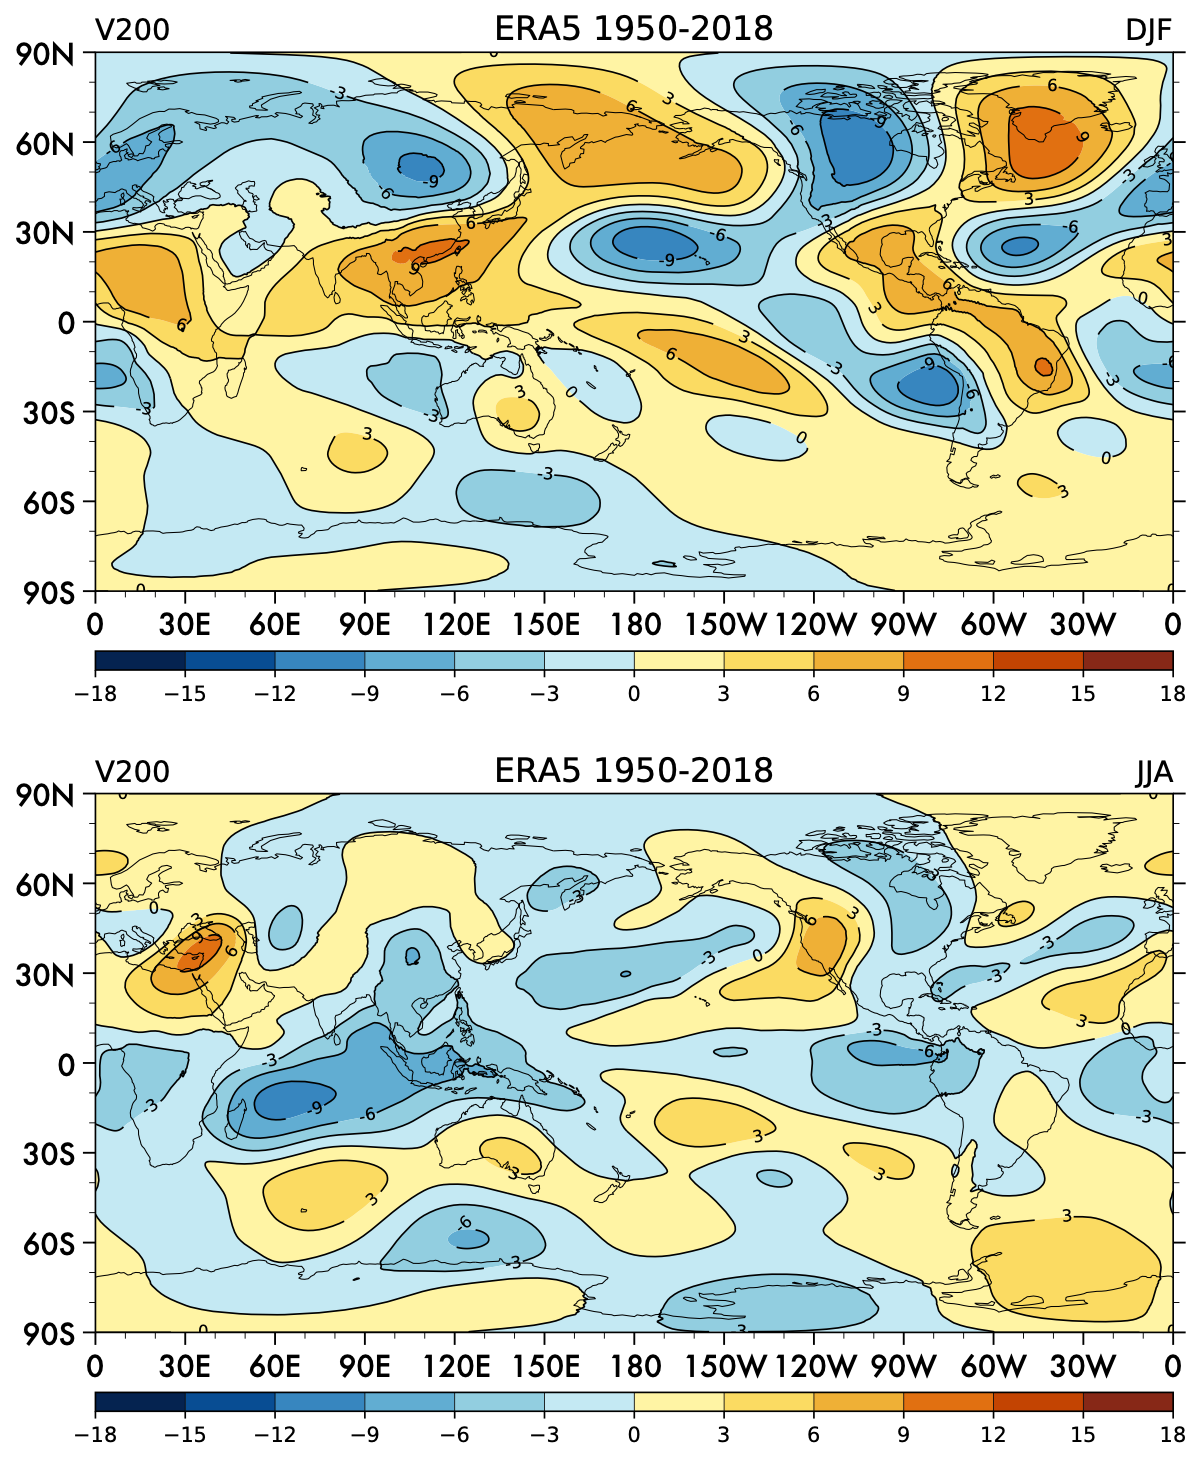
\includegraphics[width = .7 \textwidth]{figs/GD/V200.png}
\caption{}\label{}
\end{figure}

The meridional wind near the surface (Fig. \texttt{fig:58}) shows
dramatic features. Neglecting the areas of high elevation (the Himalaya
plateau, Antarctica) where this pressure level is under ground and
therefore not particularly meaningful, we notice a systematic
equatorward flow over the east coast of continents. It is most intense
along South America, South Africa and the West African coast right North
of the Equator.

In Summer these along shore winds becomes more intense along the North
American and African coast. Interestingly, the flow is reverse along thr
Somali coast in the Indian Ocean. The meridional flow is reversed with
respect the Winter season. In the Summer it is easy to see that this
flow is closing the circle with the zonal flow in Fig. \texttt{fig:55}
creating a cyclonic circulation that is the distinctive tract of the
South Asian Monsoon.

\begin{figure}
\centering
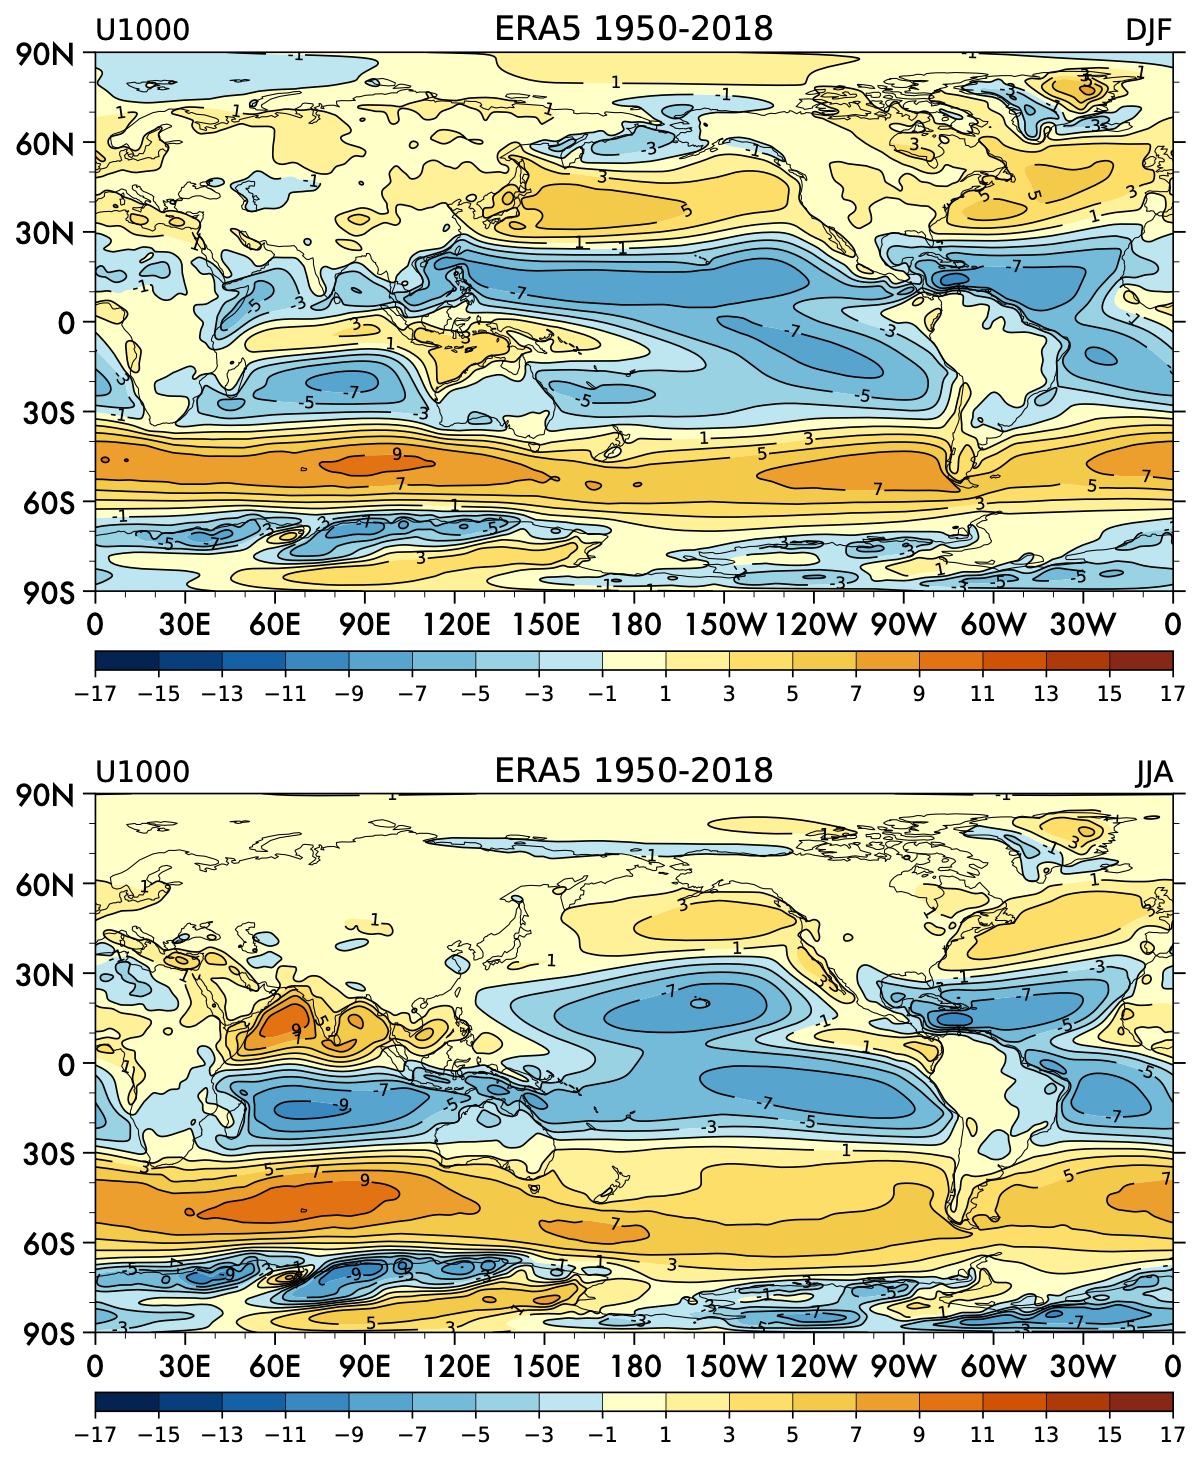
\includegraphics[width = .7 \textwidth]{figs/GD/U1000.png}
\caption{}\label{}
\end{figure}

\begin{figure}
\centering
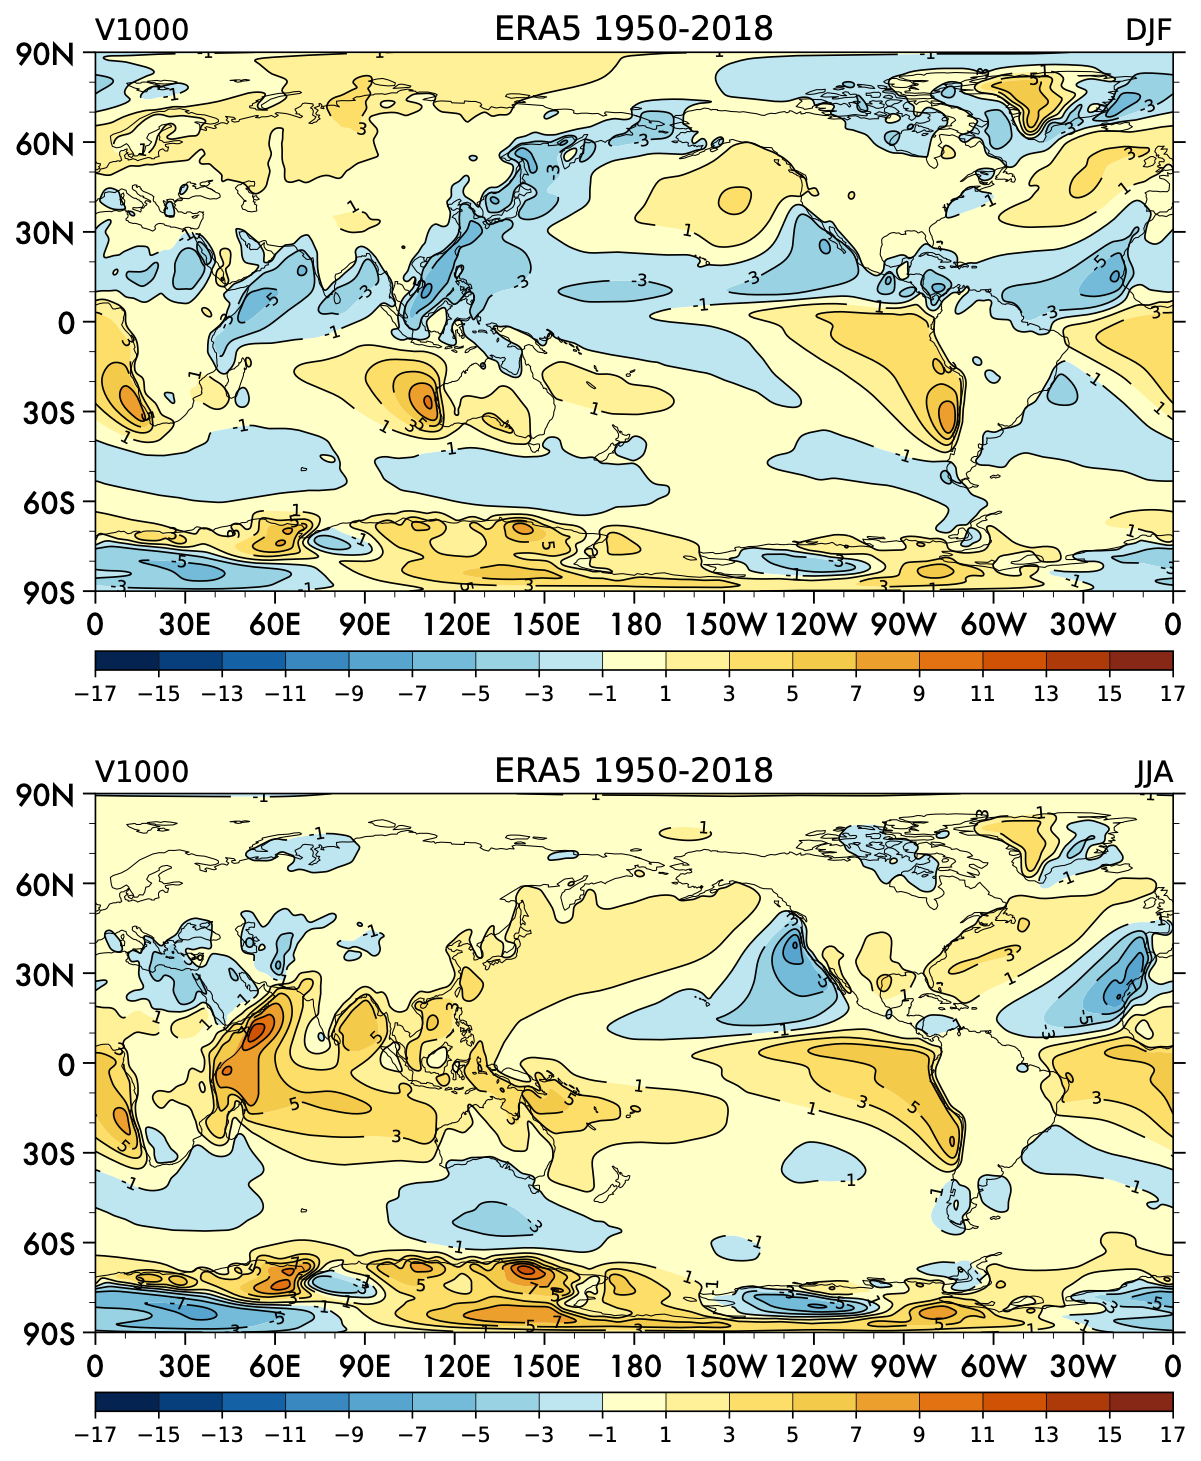
\includegraphics[width = .7 \textwidth]{figs/GD/V1000.png}
\caption{}\label{}
\end{figure}

The \(1000mb\) circulation is very close to the ground and it represent
very well the forcing that the oceans feel from the atmosphere. As such
it is a crucial element of the interactions between atmosphere and
ocean. The real low- level circulation field for the atmosphere is
better represented by a level that is outside of the planetary boundary
layer over most of the planet surface. Such a level is traditionally
considered the \(850mb\) level.

Fig. \texttt{fig:580} shows the streamlines of the wind at 850mb level
in winter and Summer. The equatorial circulation is clearly visible in
the Pacific where the Trade winds cover the equatorial region, shifting
in latitude as they follow the seasonal cycle of the ITCZ. Large gyeres
circulation covers the ocean basin and the Asian Summer Monsoon
circulation in the Indian Ocean is clearly visible, curving from the
East Africa towards the Indian subcontinent and Indochina.

\begin{figure}
\centering
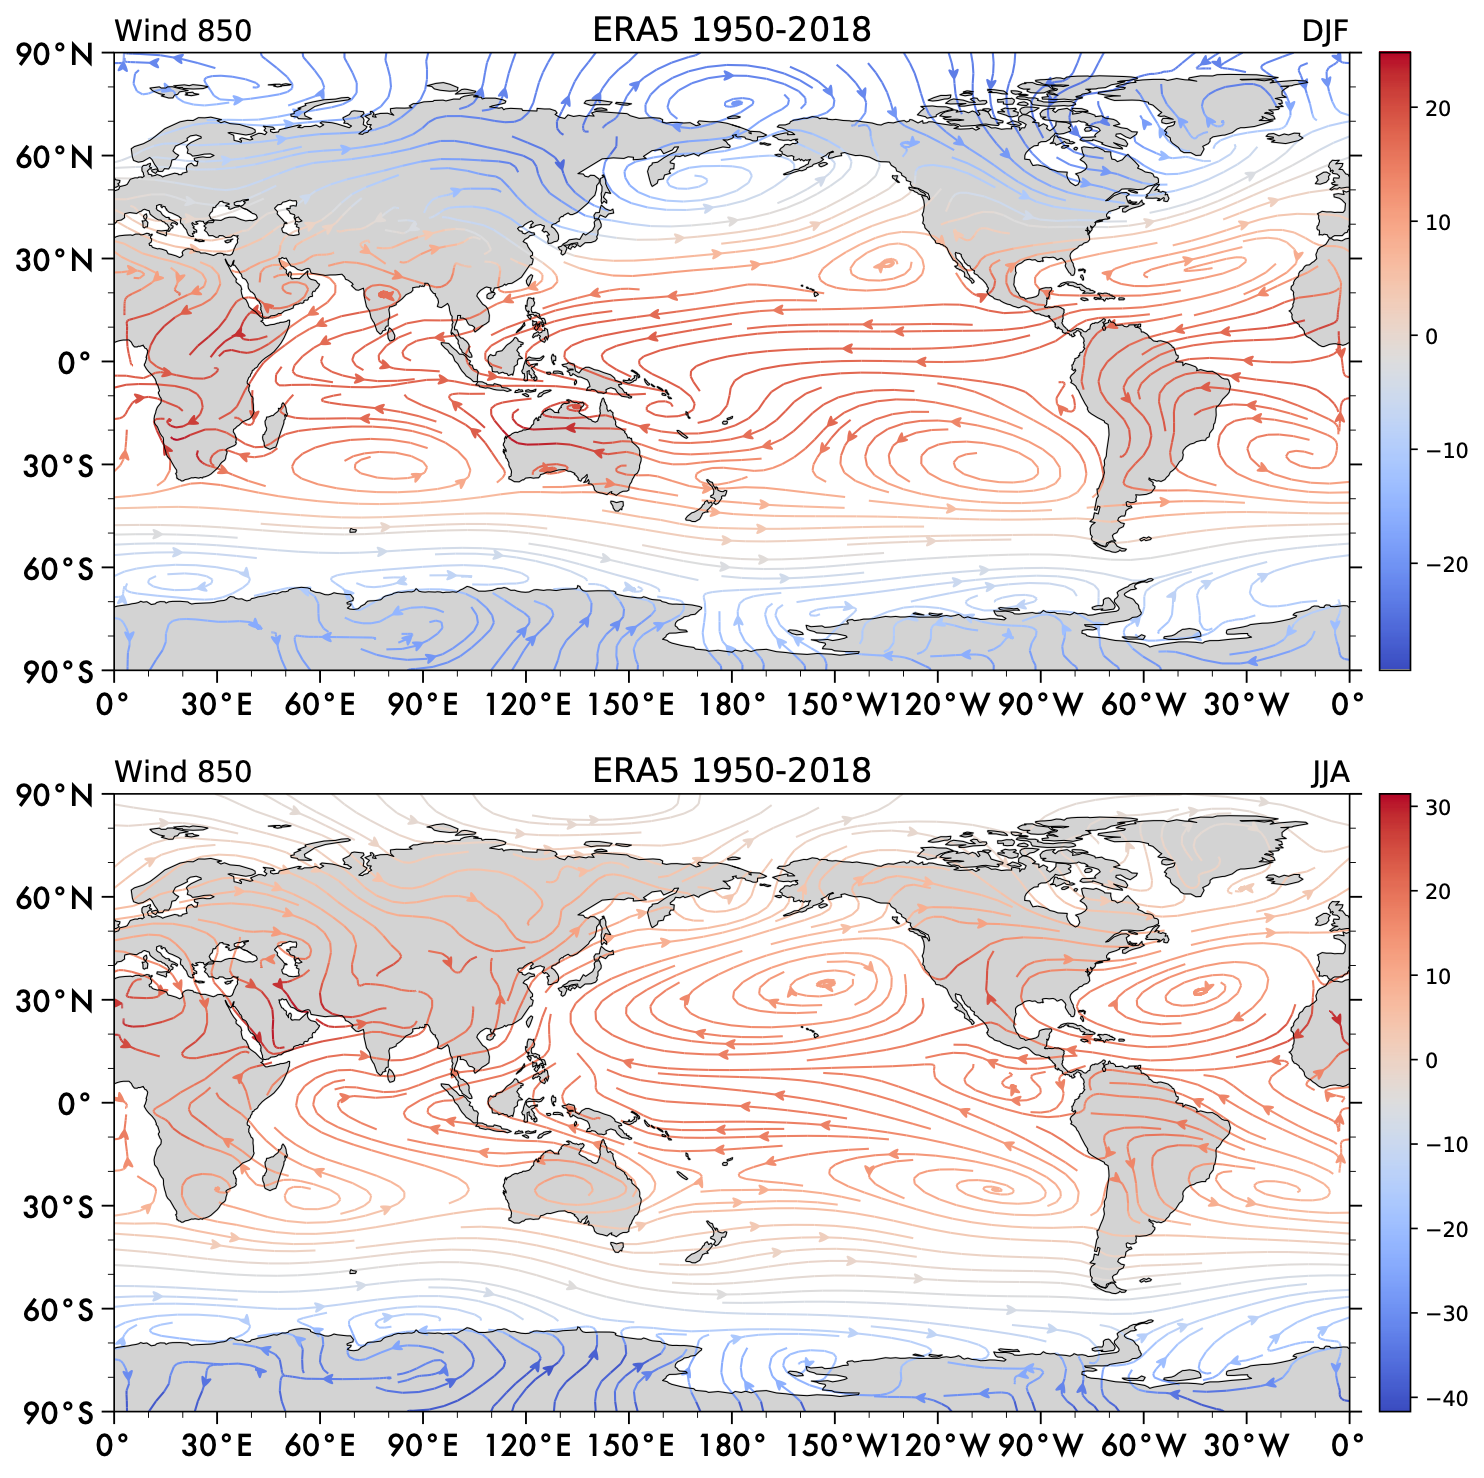
\includegraphics[width = .7 \textwidth]{figs/GD/Wind850.png}
\caption{}\label{}
\end{figure}

\subsubsection{Mean Sea Level Pressure}\label{mean-sea-level-pressure}

The distribution of Mean Sea Level pressure is another important
parameter to describe the general circulation of the atmosphere. This
field is obtained by calculating the pressure at the reference level for
the geopotential (zero level) that is conventionally considered the mean
sea level. It should better referred to as the reference geoid, but most
models still use a spherical Earth approximation, so the zero reference
can still be defined as a sphere.

The principal throwback is that this means that the areas of the Earth
where there are mountains the mean sea level is effectively underground
and therefore of limited usefulness. This especially evident for the
high mountain ranges, the Rockies and the Himalayas and for Antarctica.
Elsewhere, however, it gives a good description of the mass distribution
of the atmosphere. High values of mean sea level pressure correspond to
pile up of mass. The accumulation of mass is larger in the subtropics,
both in Winter and Summer, where a chain of high pressure centers is
present.

The picture is that there are three distinctively different region. The
Northern Hemisphere Midlatitudes, the intertropical region between the
Tropics and the midlatitudes of the Southern Hemisphere. The largest
seasonal contrast emerges in the northern hemisphere mid latitudes. Note
that in Winter high pressure tend to stay over the continent, whereas
low pressure centers develop over the ocean, in Summer it is the
opposite and high pressure stays over the continents.

The Intertropical zone is characterized by the presence of distinct high
pressure centers that oscillate with the season in latitude. The
Southern Hemisphere has a much more symmetric nature with a ring of low
pressure circling the Antarctic continent.

The seasonal cycle is visible in the shift of the ring of high pressure
at the rtropics in the north-south directions. Fig. \texttt{fig:59z}
shows the zonal and time mean for Summer and Winter of the meridional
distribution of sea level pressure. There is a general structure of high
sea level pressure in the tropics, with relative areas of low pressure
in the mid-latitudes and at the Equator. In the Southern hemisphere it
is ismuch more pronounced andf the gradients are much stronger. The
seasonal shift can be seen in the movement of tropical maxima.

\begin{figure}
\centering
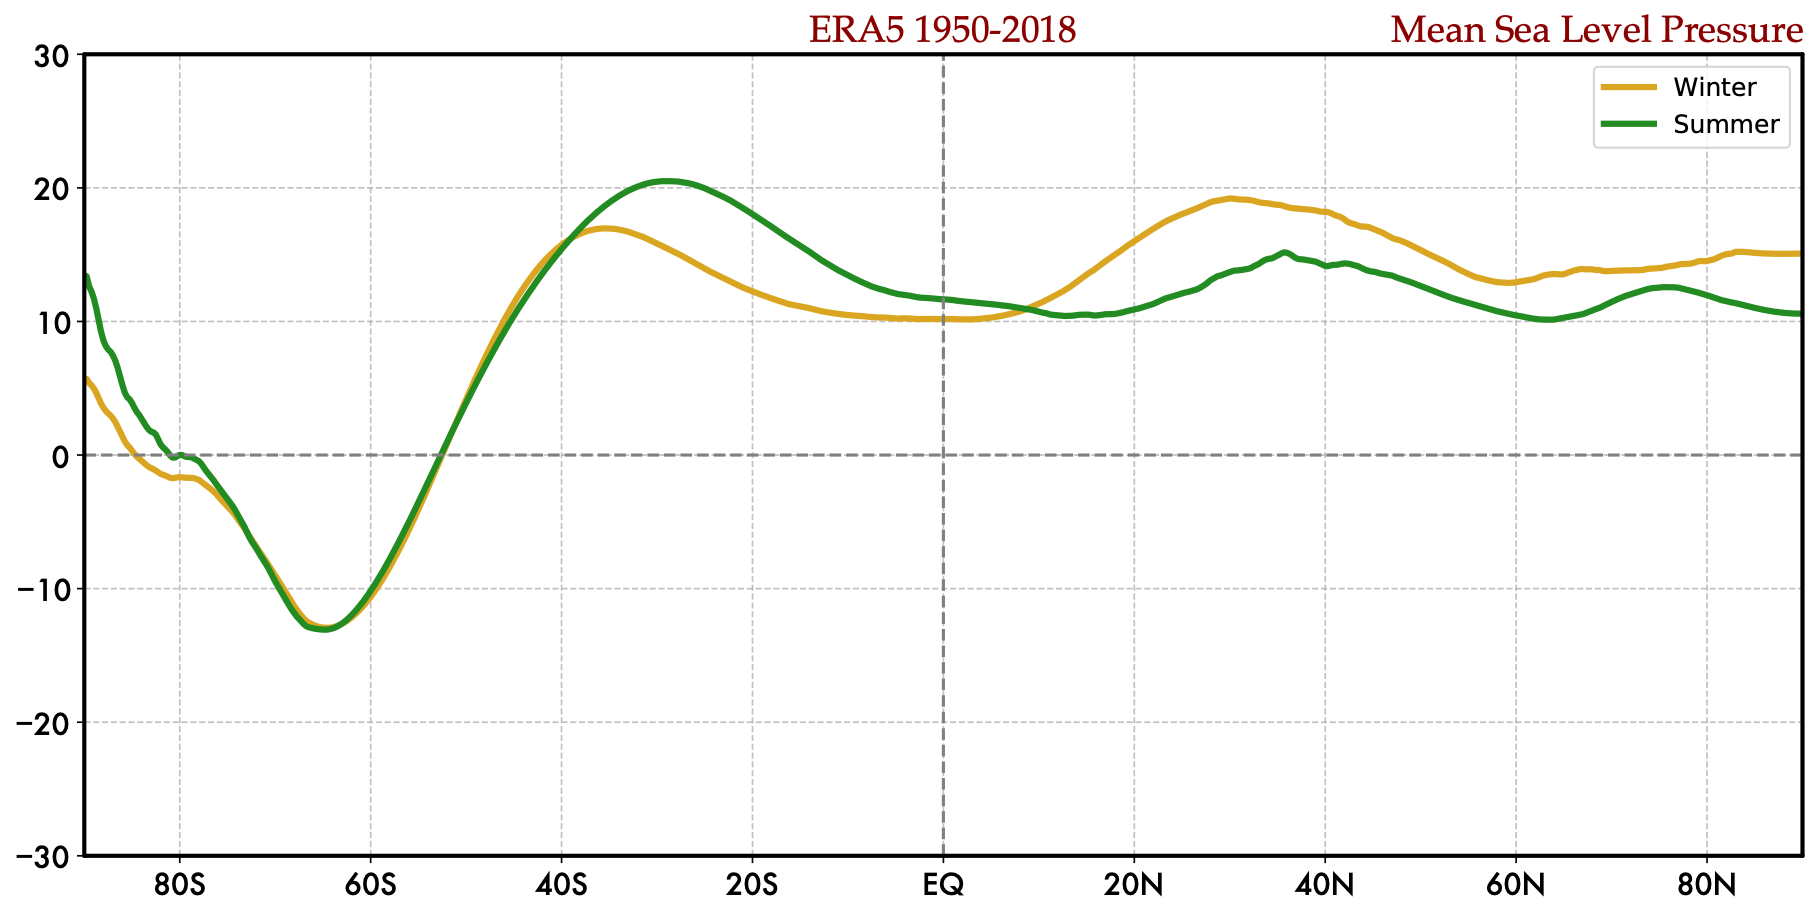
\includegraphics[width = .7 \textwidth]{figs/GD/MSLZONALLDJF.png}
\caption{}\label{}
\end{figure}

\subsubsection{The Sea Surface
Temperature}\label{the-sea-surface-temperature}

North-South gradients dominate the distribution of the Sea Surface
Temperature in both seasons (Fig. \texttt{fig:60}). Polar regions are
very cold and dominated by sea ice (not visible in this picture),
whereas the equatorial regions are generally very warm. However, there
are large deviation from the zonal symmetry close to the east cost of
continents. especially in the equatorial Pacific Ocean vast intrusions
of cold water are visible straight at the equator in the East Pacific,
where the water has the same temperature of the midlatitudes.

\begin{figure}
\centering
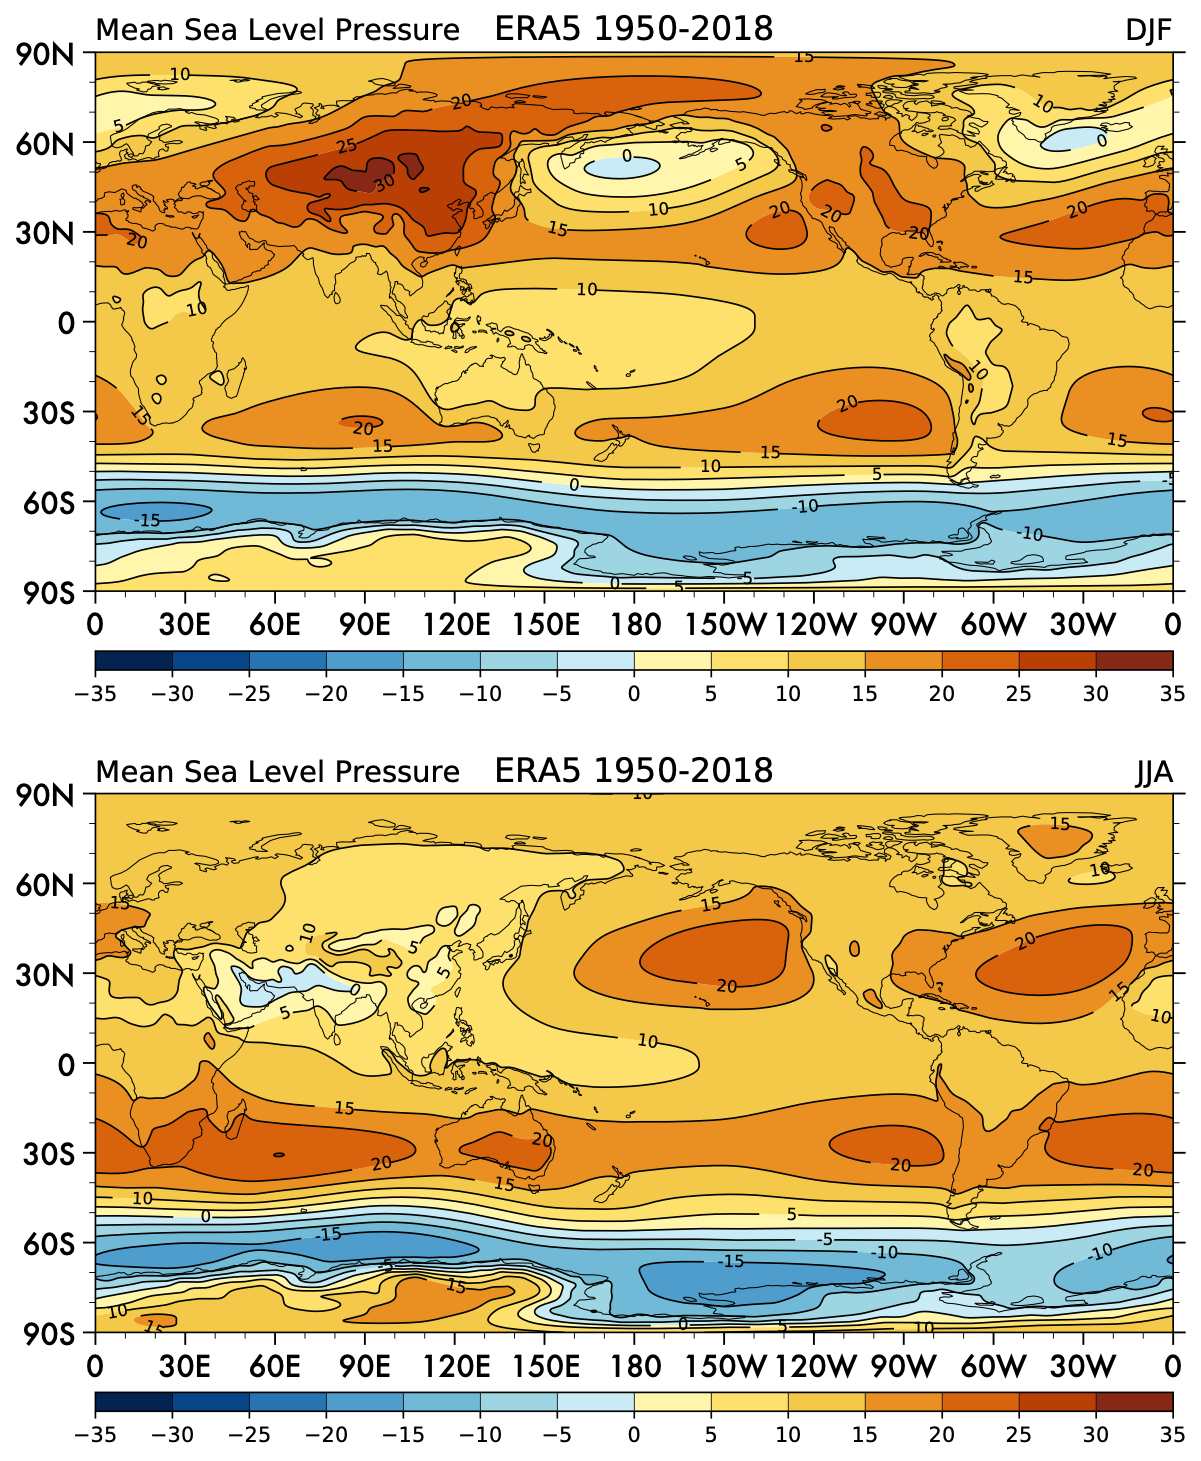
\includegraphics[width = .7 \textwidth]{figs/GD/MSL.png}
\caption{}\label{}
\end{figure}

This is in contrast with the West Pacific where a pool of very warm
water cover the entire region. it is clear that a large gradients exist
also at the surface along the Equator in the SST.

\begin{figure}
\centering
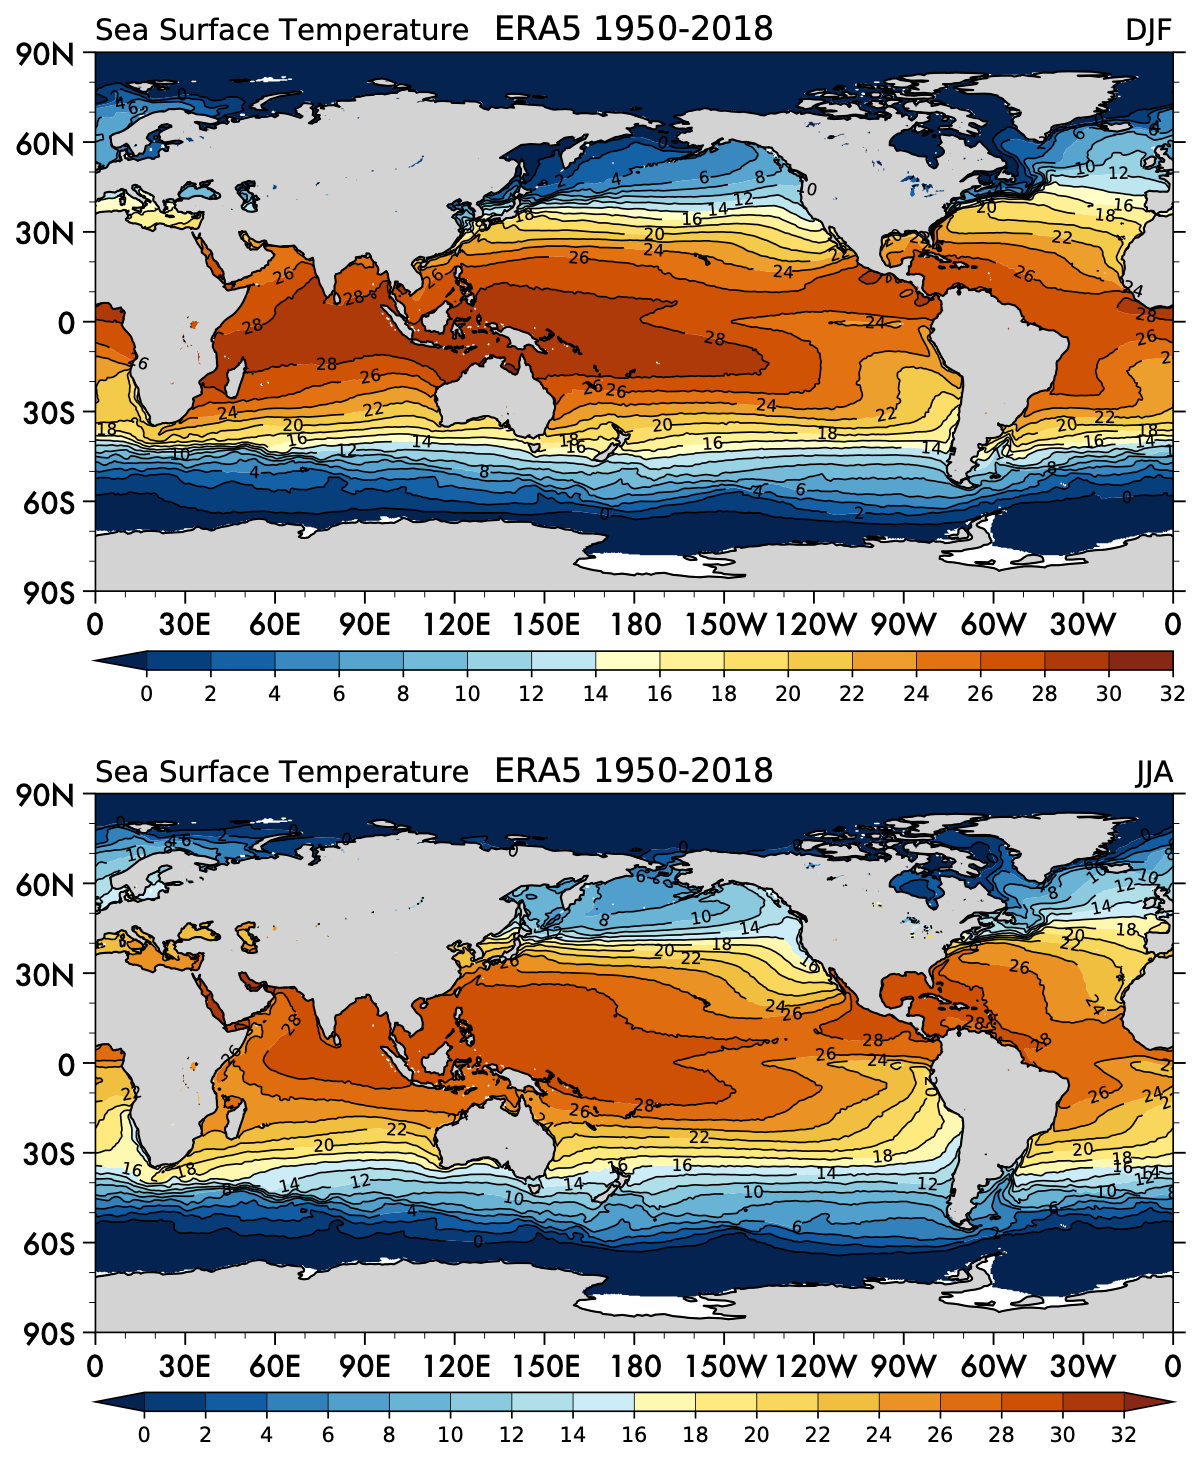
\includegraphics[width = .7 \textwidth]{figs/GD/SST.png}
\caption{}\label{}
\end{figure}

\subsubsection{The 2 Meter Temperature}\label{the-2-meter-temperature}

The SST show clearly the structure of the surface of the ocean, but it
is important to look also at near surface temperature for the entire
Earth surface. Land temperature will adjust very rapidly to the energy
balance and so it is usually used as a parameter of the surface
temperature the air temperature very close to the surfcae, usually
defined at two meter above the local surface. (Fig. \texttt{fig:602T})
show this temperature for Summer (bottom) and Winter (top). Over the
oceans it follows the SST as before, but over the continent it show a
strong seasonal variation. The northern continents are significantly
colder than the oceans at the same latitude. The West coasts of
continents is also relatively milder than the East Coasts.

\begin{figure}
\centering
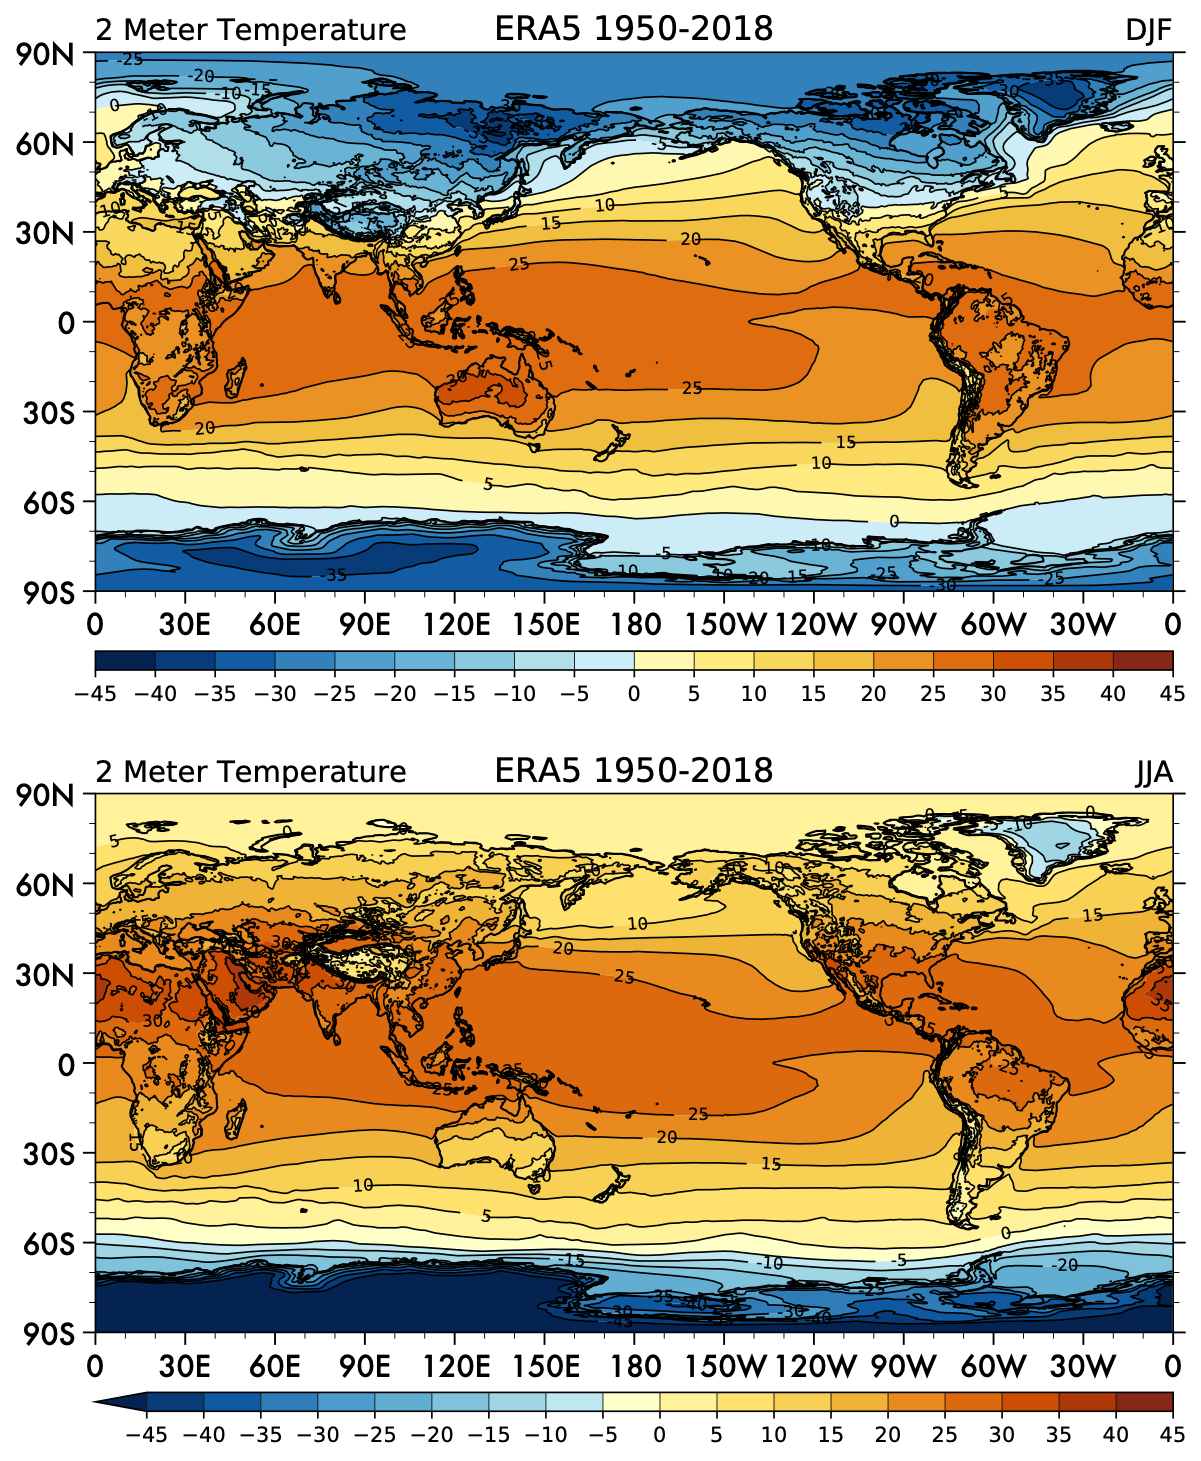
\includegraphics[width = .7 \textwidth]{figs/GD/2T.png}
\caption{Two Meter Air temperature for DJF (top) and JJA (bottom).}
\label{fig:}
\end{figure}

This is in contrast with the West Pacific where a pool of very warm
water cover the entire region. it is clear that a large gradients exist
also at the surface along the Equator in the SST.

\subsection{The Kinetic Energy}\label{the-kinetic-energy}

The total kinetic energy per unit mass can be defined as

\[K_T = \frac{1} {2} ( u^2 + v^2).\]

We can analyze the contribution of different components introducing the
splitting \((u = \bar{u}+ u', \cdots )\) for the time mean and similarly
for the zonal mean and following the arguments in Section
\texttt{Sect:Higher}, we get

\[K_T = \frac{1} {2}( [\overline{u^2} + \overline{v^2}])\]

where

\[\begin{aligned}
&K_{SE} =\frac{1} {2}( [(\bar{u}^*)^2]  + [(\bar{v}^*)^2]) \qquad & \text{Stationary Eddies}\\
& K_{TE} = \frac{1} {2}( [\overline{u'^2}]  +[\overline{v'^2}] ) \qquad & \text{Transient Eddies}\\
& K_{MME} = \frac{1)} {2}([\bar{u}]^2 + [\bar{v}]^2) \qquad & \text{Mean Meridional Circulation}
\end{aligned}\]

The largest contribution comes from the meridionally symmetric component
(\(K_{MME}\) -- top panel). This is consistent with the weaker eddy
stationary component in this region, resulting in a more symmetric,
almost annular jet. The dominance of this component of course is one of
the reason under the observation of the \emph{circumpolar jet} as the
basic paradigm of the global circulation.

We present in Fig. :numref\texttt{fig:705} the kinetic energy split for
DJF and JJA. The calculation has been performed on the monthly mean data
from ERA5 therefore the transient elements are to be understood as
transients with respect the monthly mean variation from one month to
another. The data are then averaged over the season.

The transients contribution (\(K_{TE}\) -- second panel) is localized at
the margin of the subtropical zone with a visible extension into the
midlatitudes, basically it is confined between 30N and 60N. It is also
to be noted that these statistics were computed from monthly means data
and therefore some transients is being smoothed by the monthly mean.
Once again we can see here the effect of choosing a particular averaging
period.

The next term \(K_{SE}\) represents the contribution to the kinetic
energy of the time mean (stationary) deviations from the zonal mean
(eddies). The contribution from the standing eddies is large, indicating
a strong tendency of the Northern Hemisphere to generate slow, coherent
eddy structures that tend to persist on the monthly time scale.

\begin{figure}
\centering
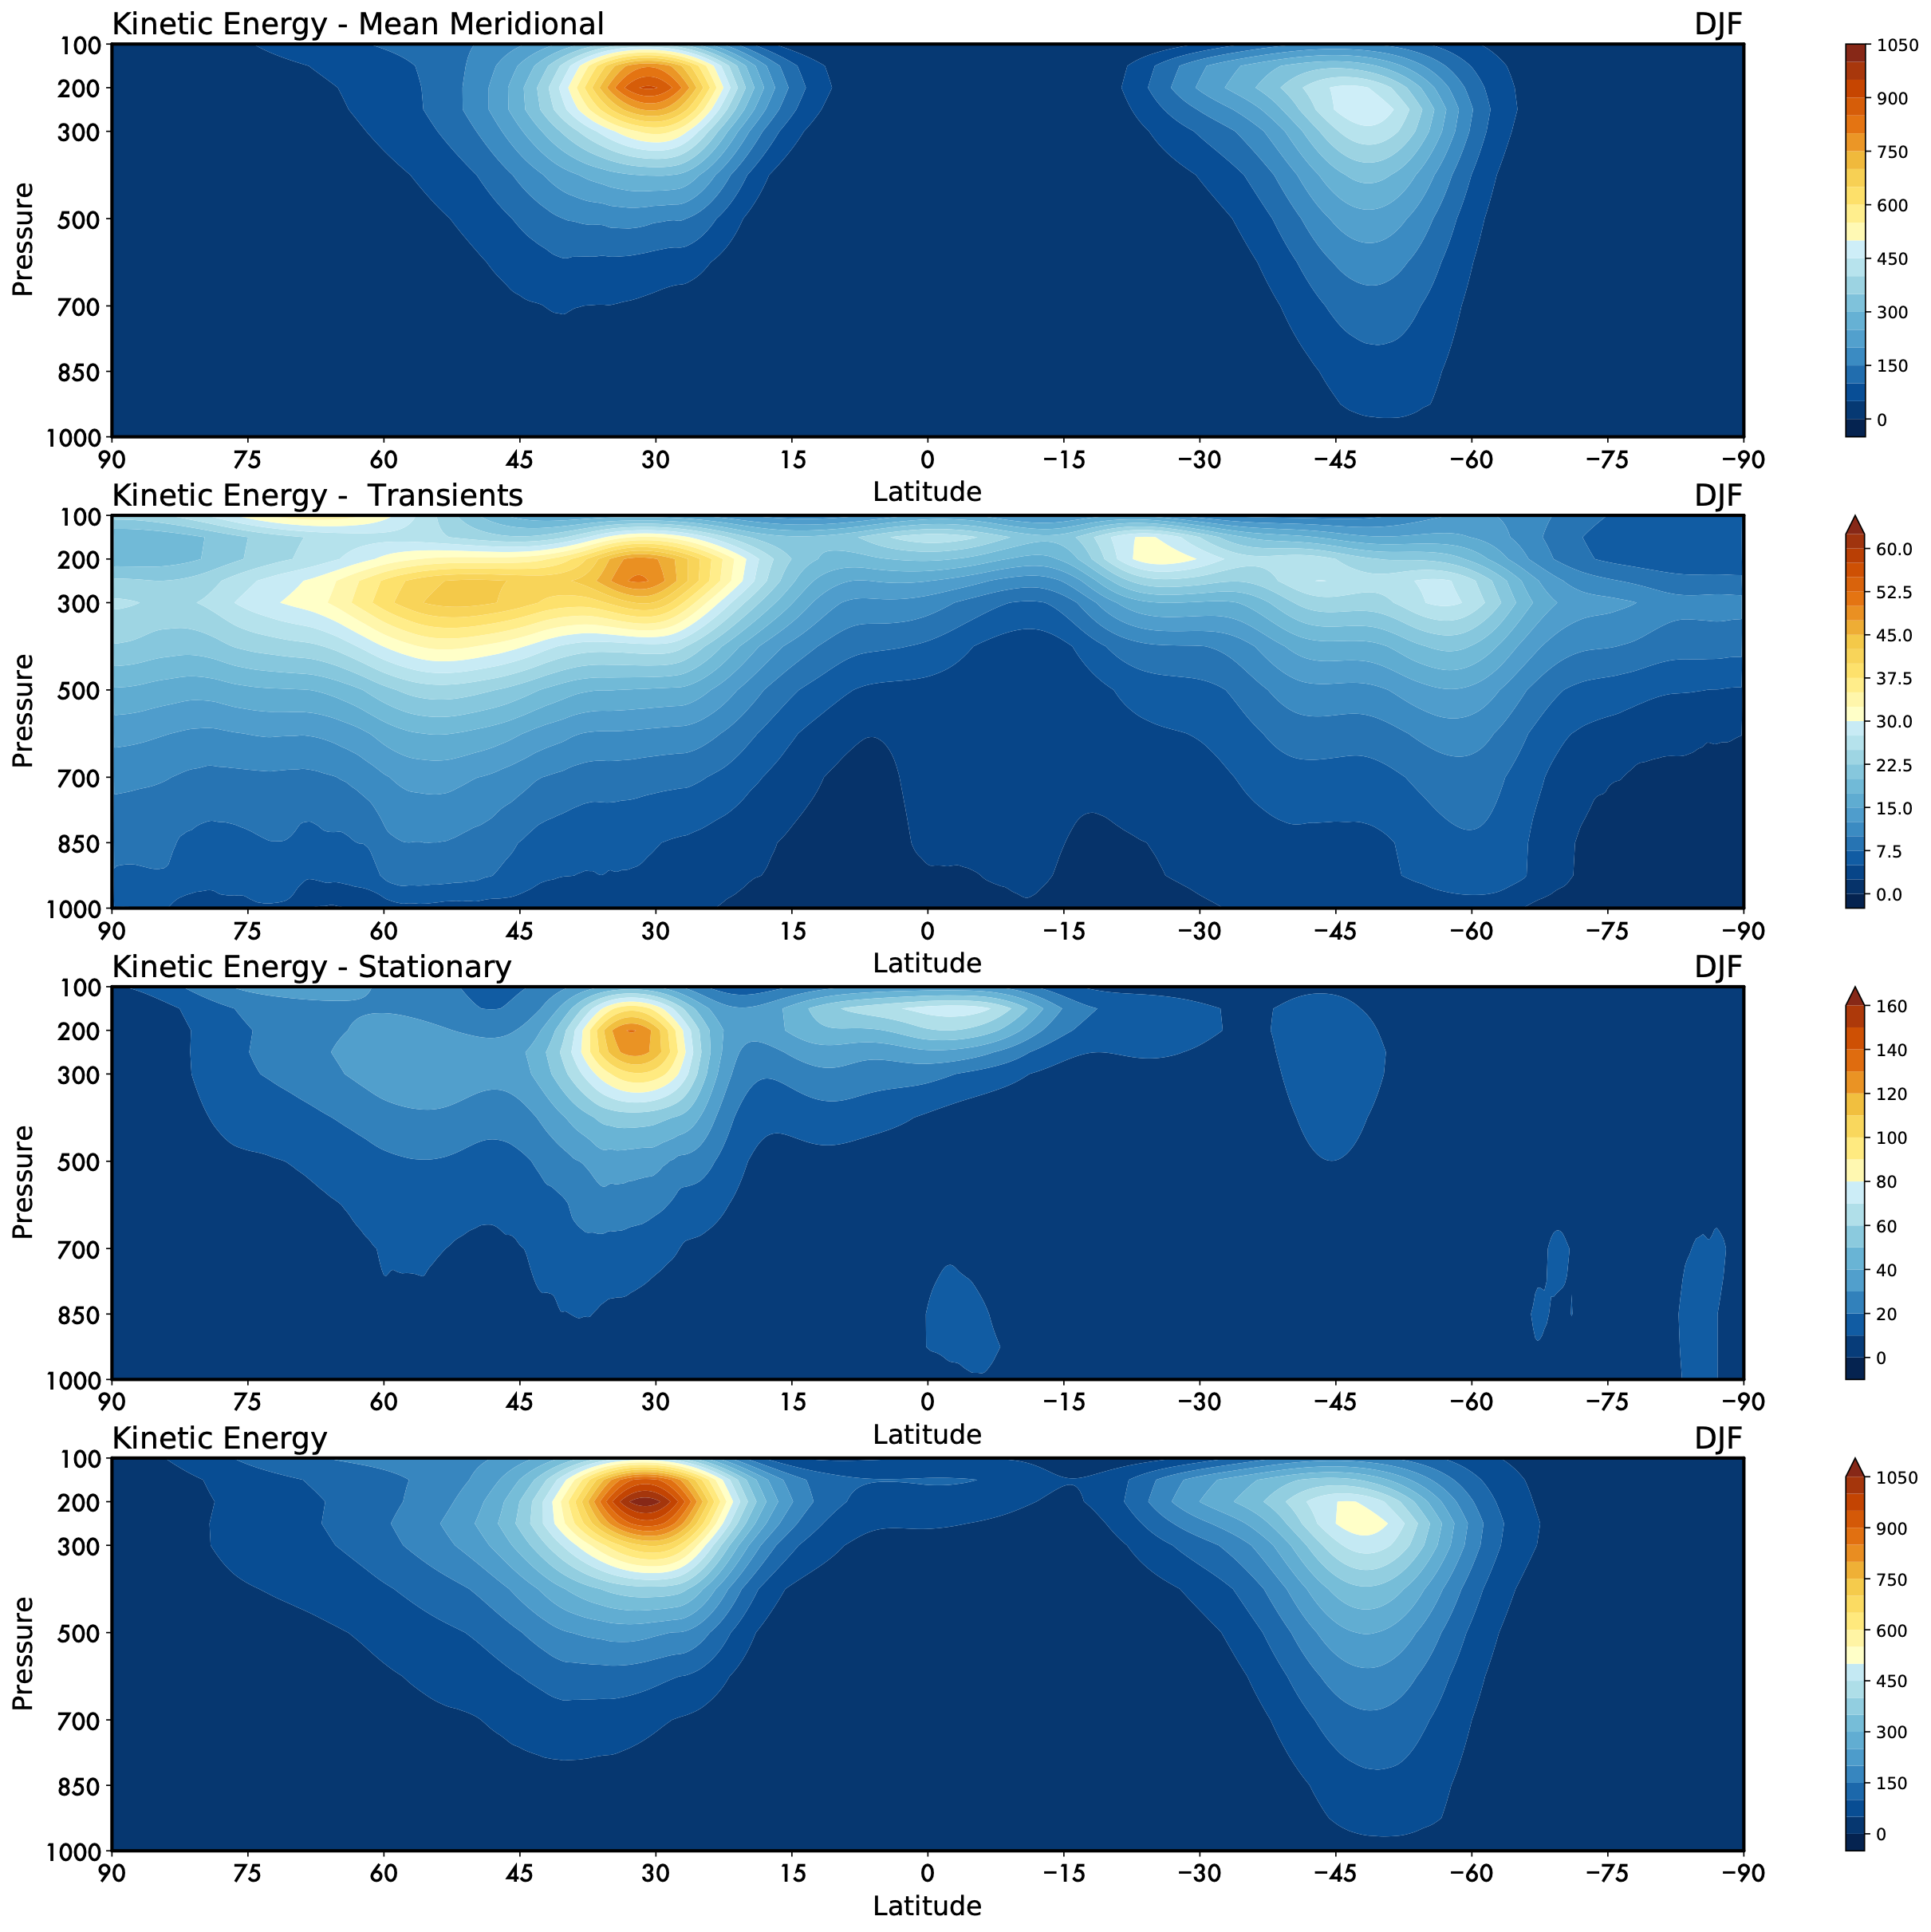
\includegraphics[width = .7 \textwidth]{figs/GD/DJFKEFlux.png}
\caption{}\label{}
\end{figure}

And finally the total kinetic energy \(K_T\) in northern hemisphere
Winter (bottom panel of Fig. \texttt{fig:70}) , shows a clear
correlation in the location of the zonal jets, both in latitude and
altitude.

\begin{figure}
\centering
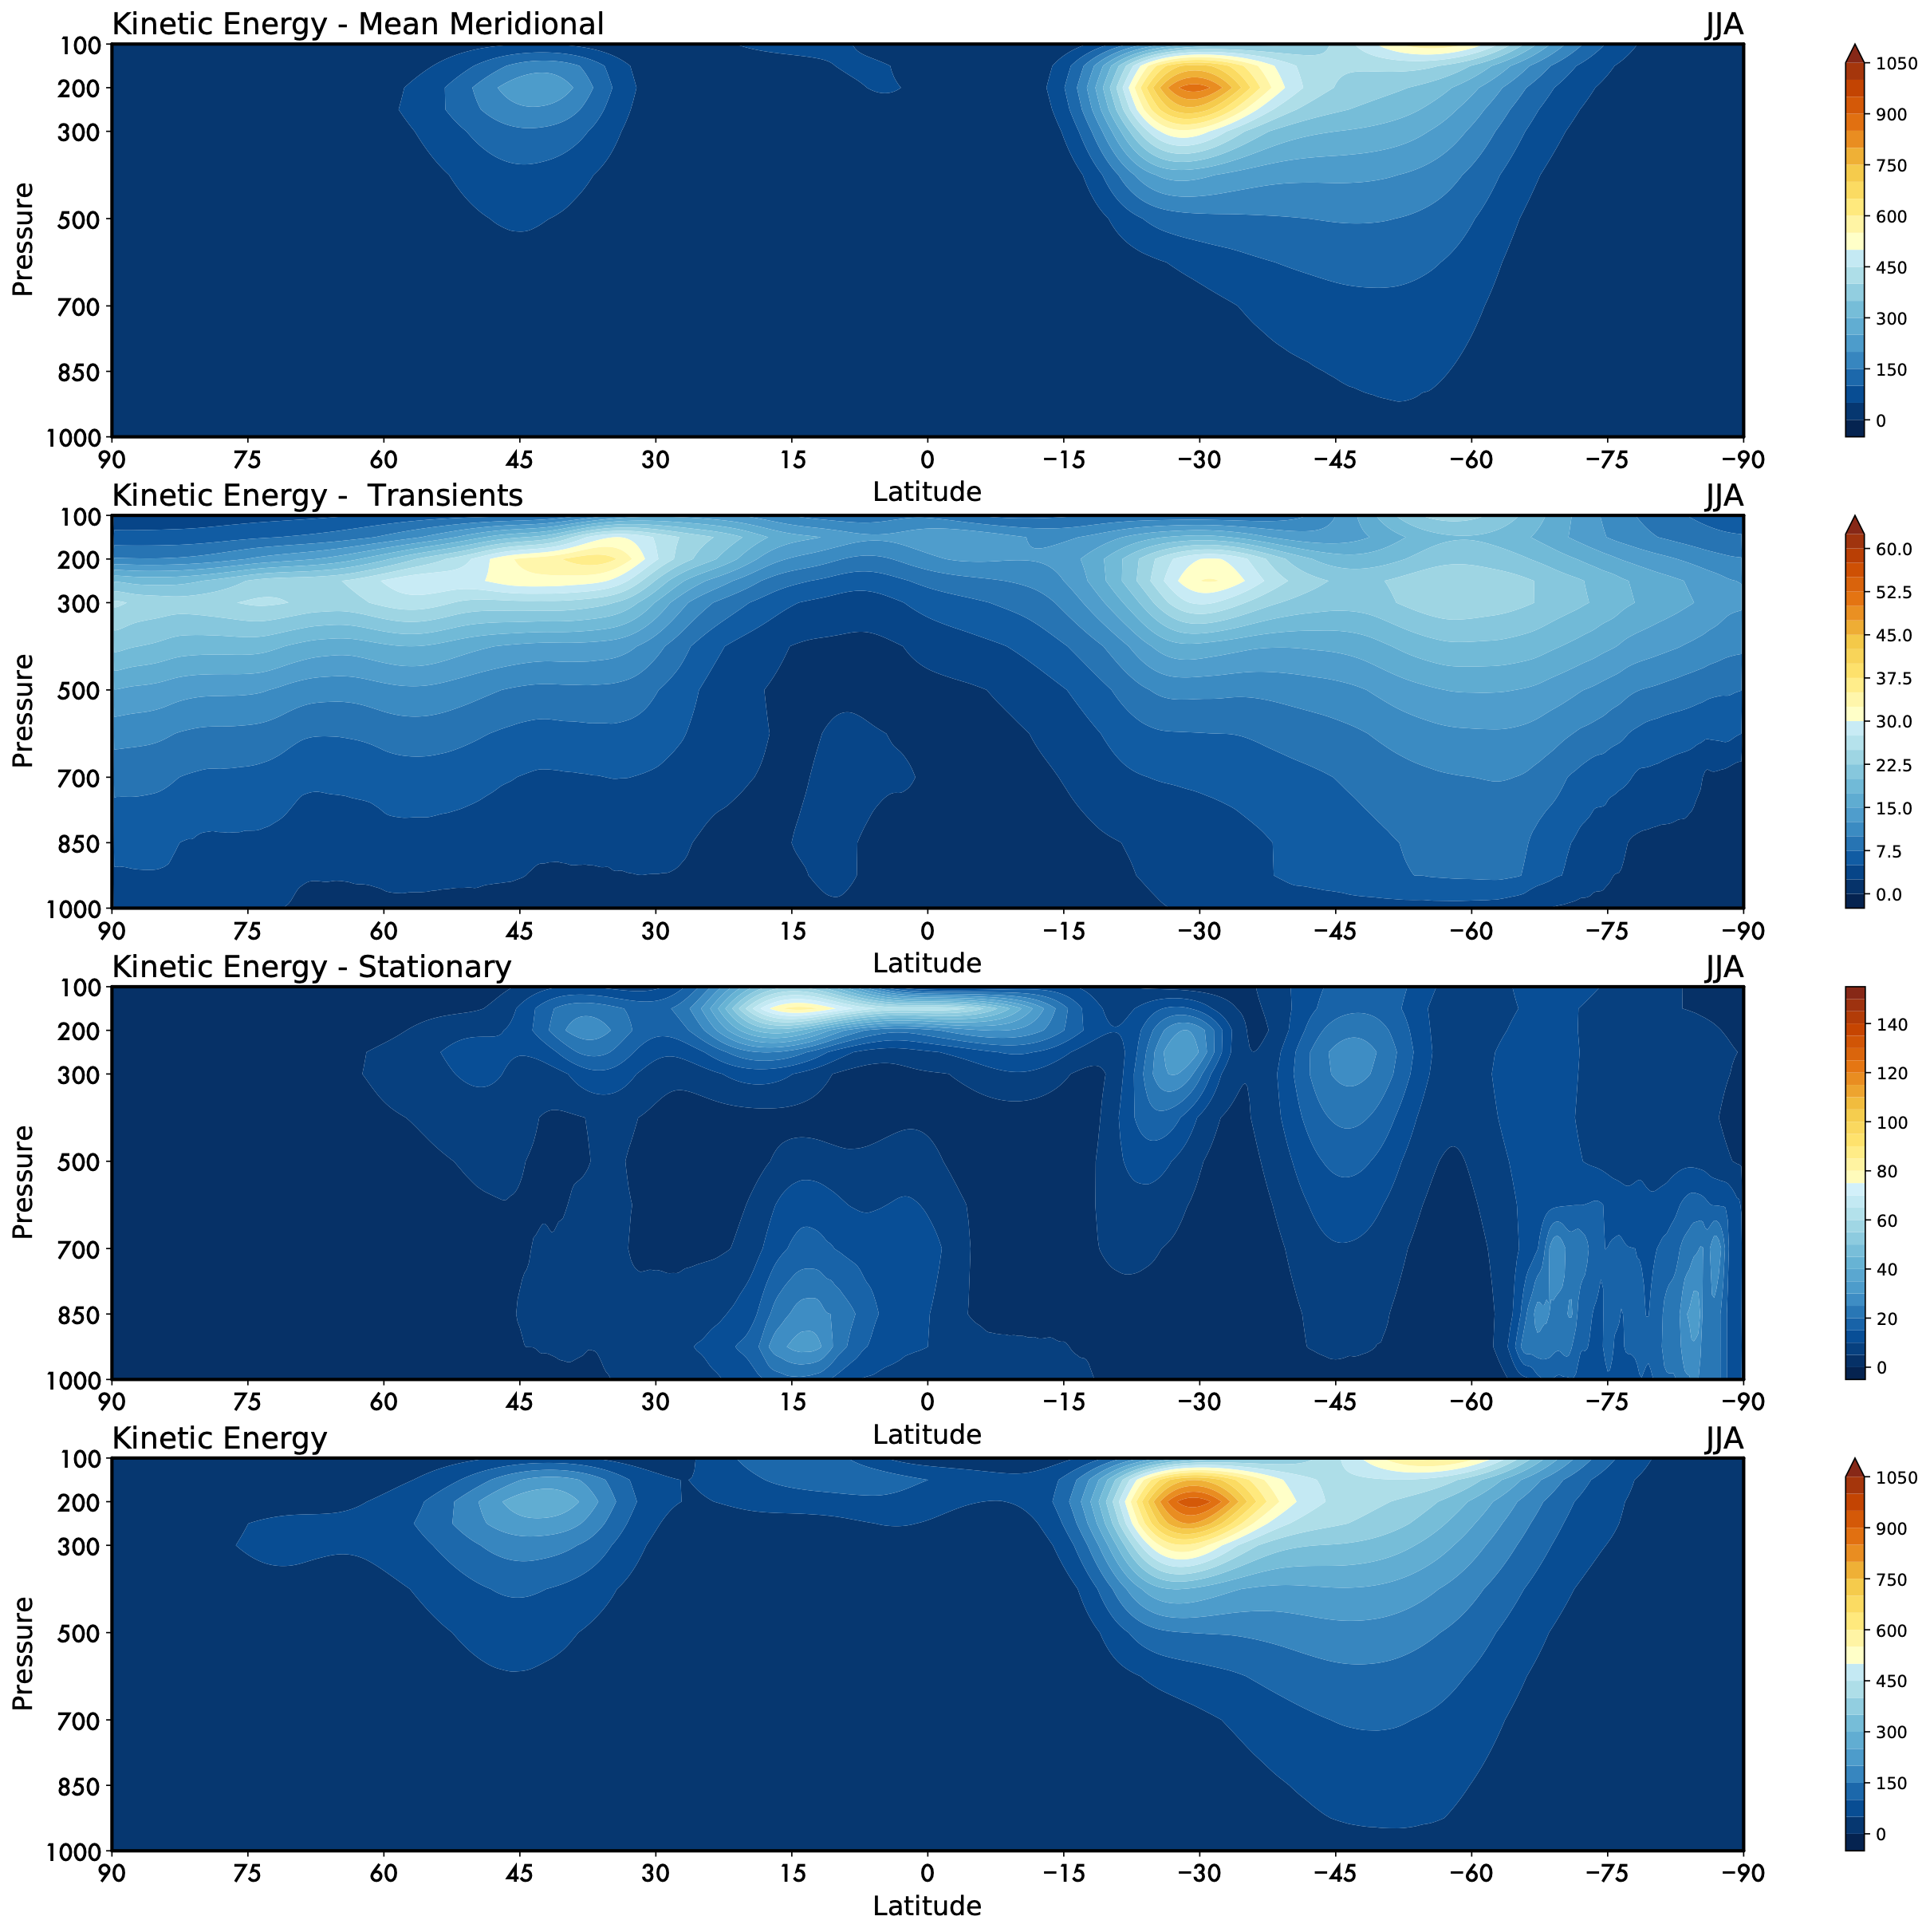
\includegraphics[width = .7 \textwidth]{figs/GD/JJAKEFlux.png}
\caption{}\label{}
\end{figure}

A similar situation is described in \texttt{fig:705} for JJA. Also in
this case the kinetic energy is colocated with the jet locations, but it
is possible to see that the standing eddies (third panel) are weaker
than in the Northern Hemisphereand a certain amount of transients is
still present in the Northern Hemisphere.

\subsection{The Meridional Momentum
Flux}\label{the-meridional-momentum-flux}

\begin{figure}
\centering
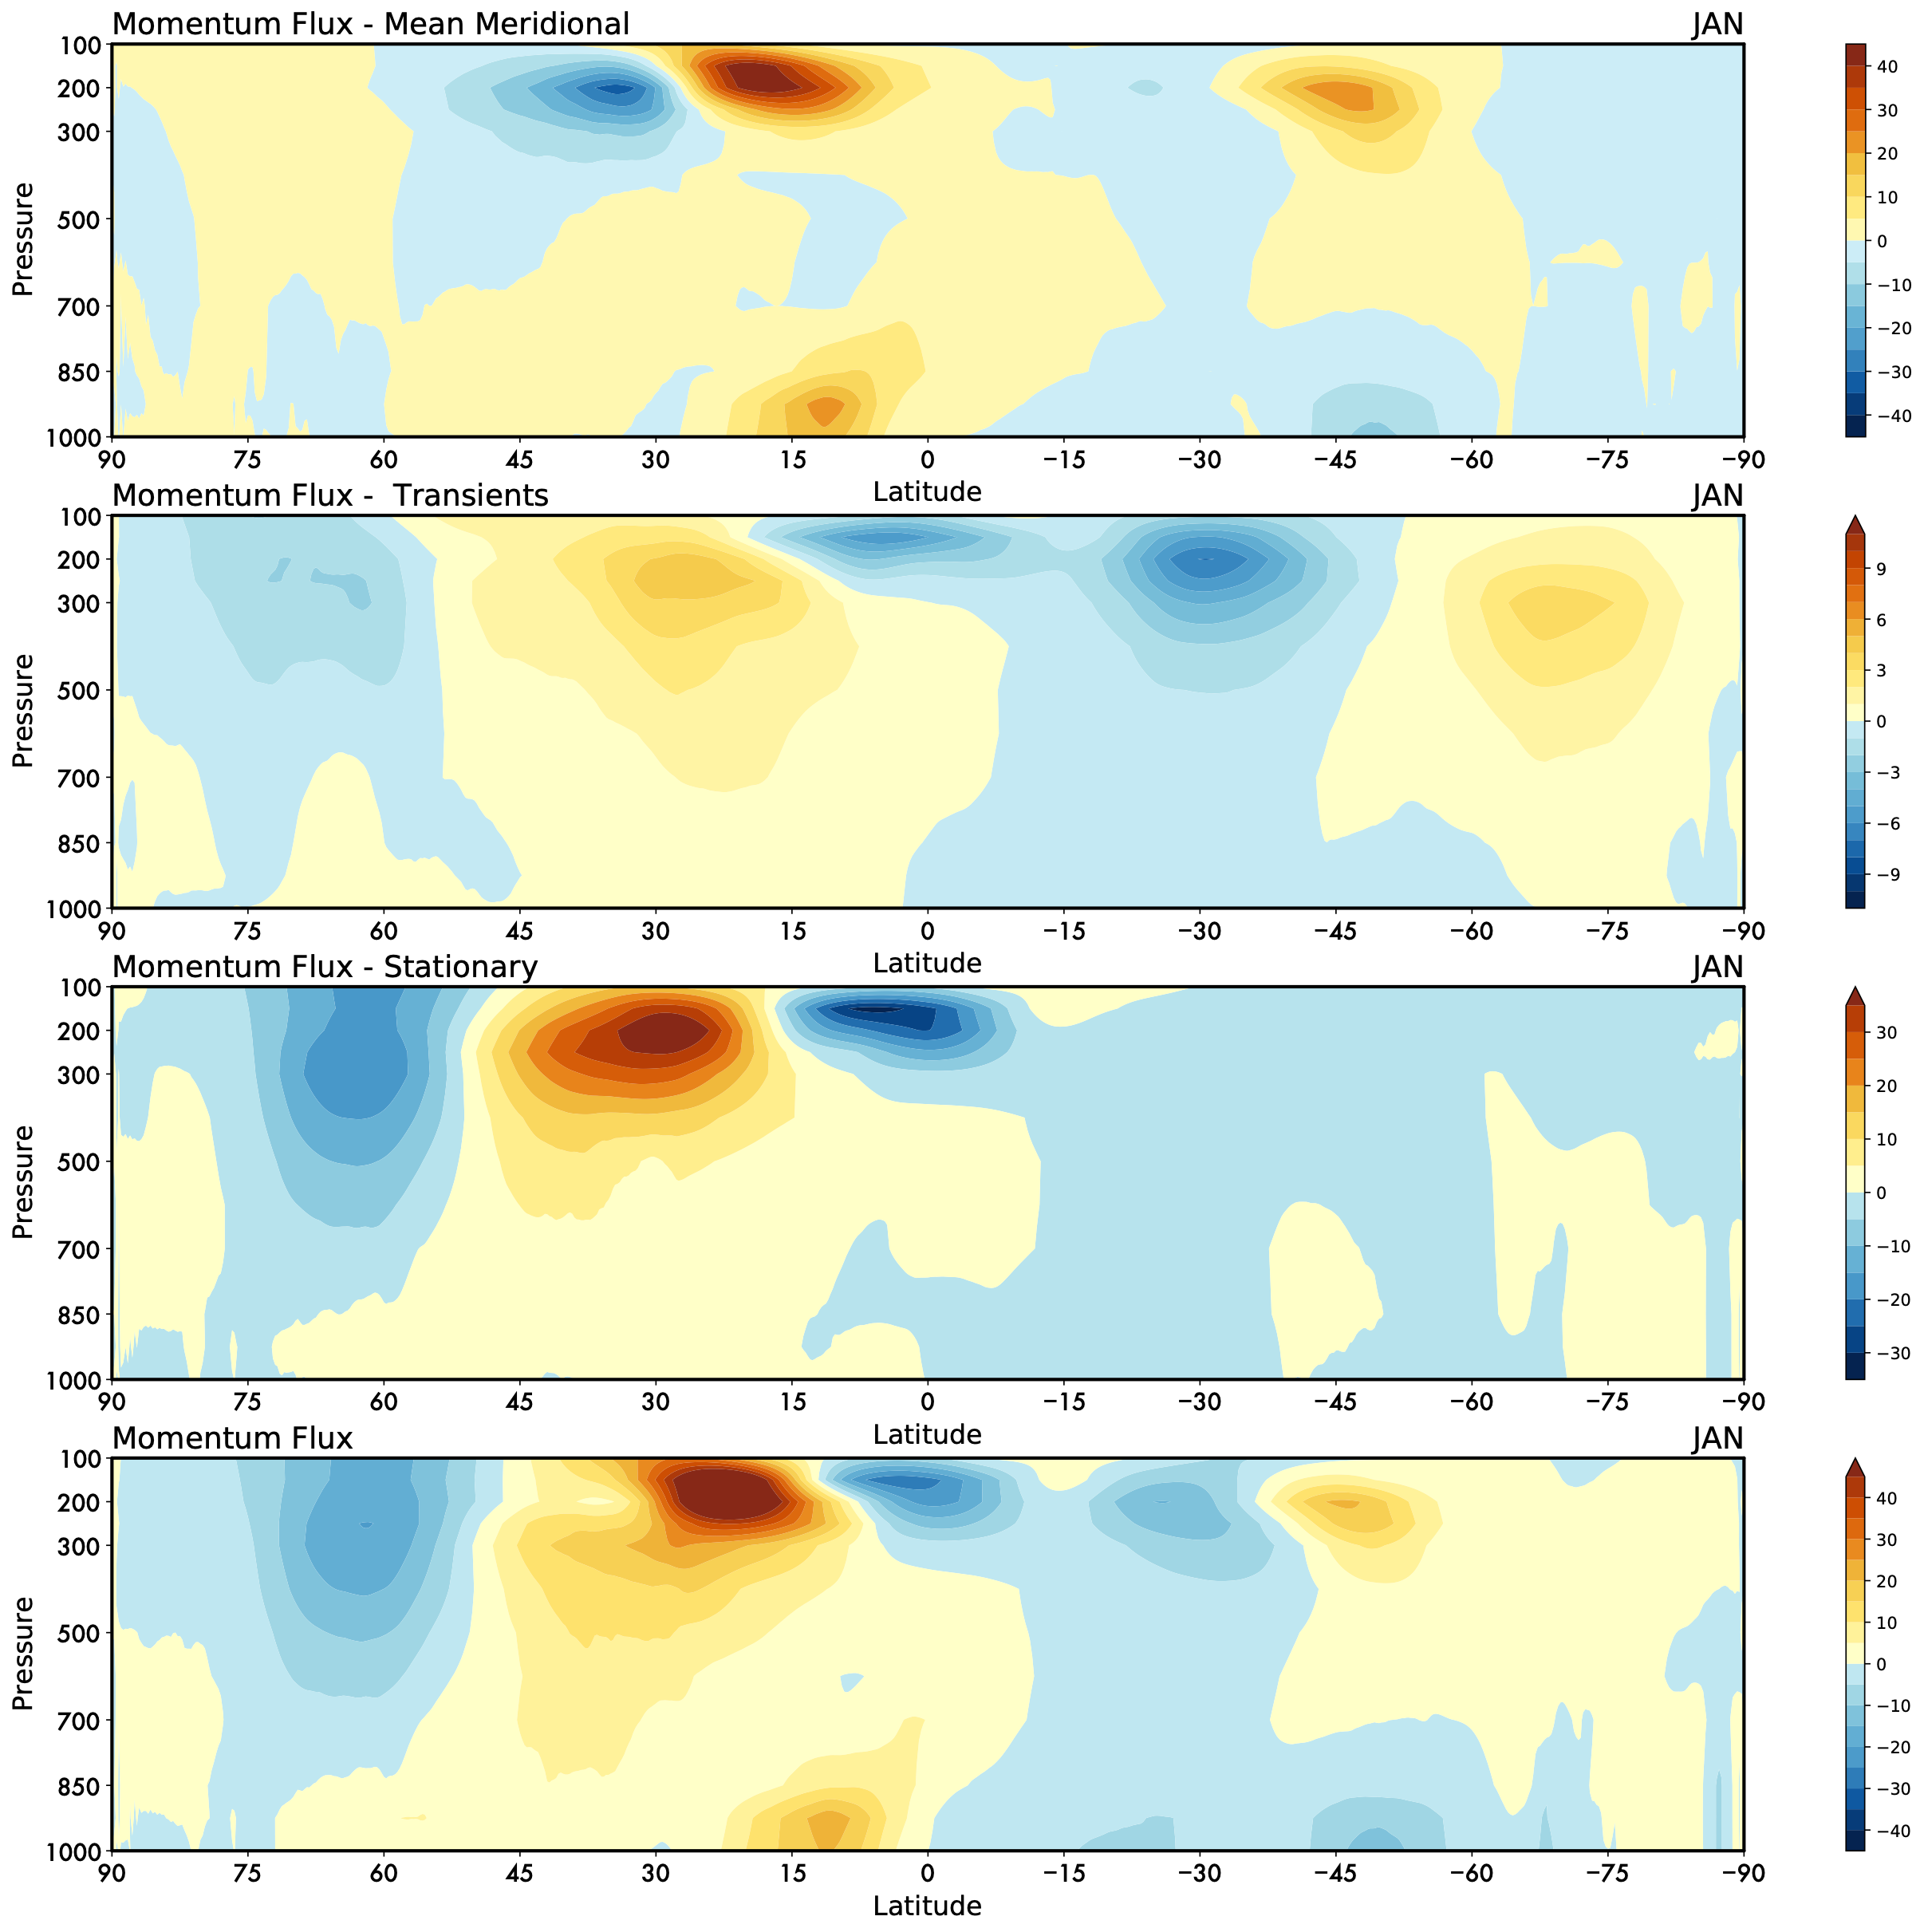
\includegraphics[width = .7 \textwidth]{figs/GD/JANUVFlux.png}
\caption{}\label{}
\end{figure}

\begin{figure}
\centering
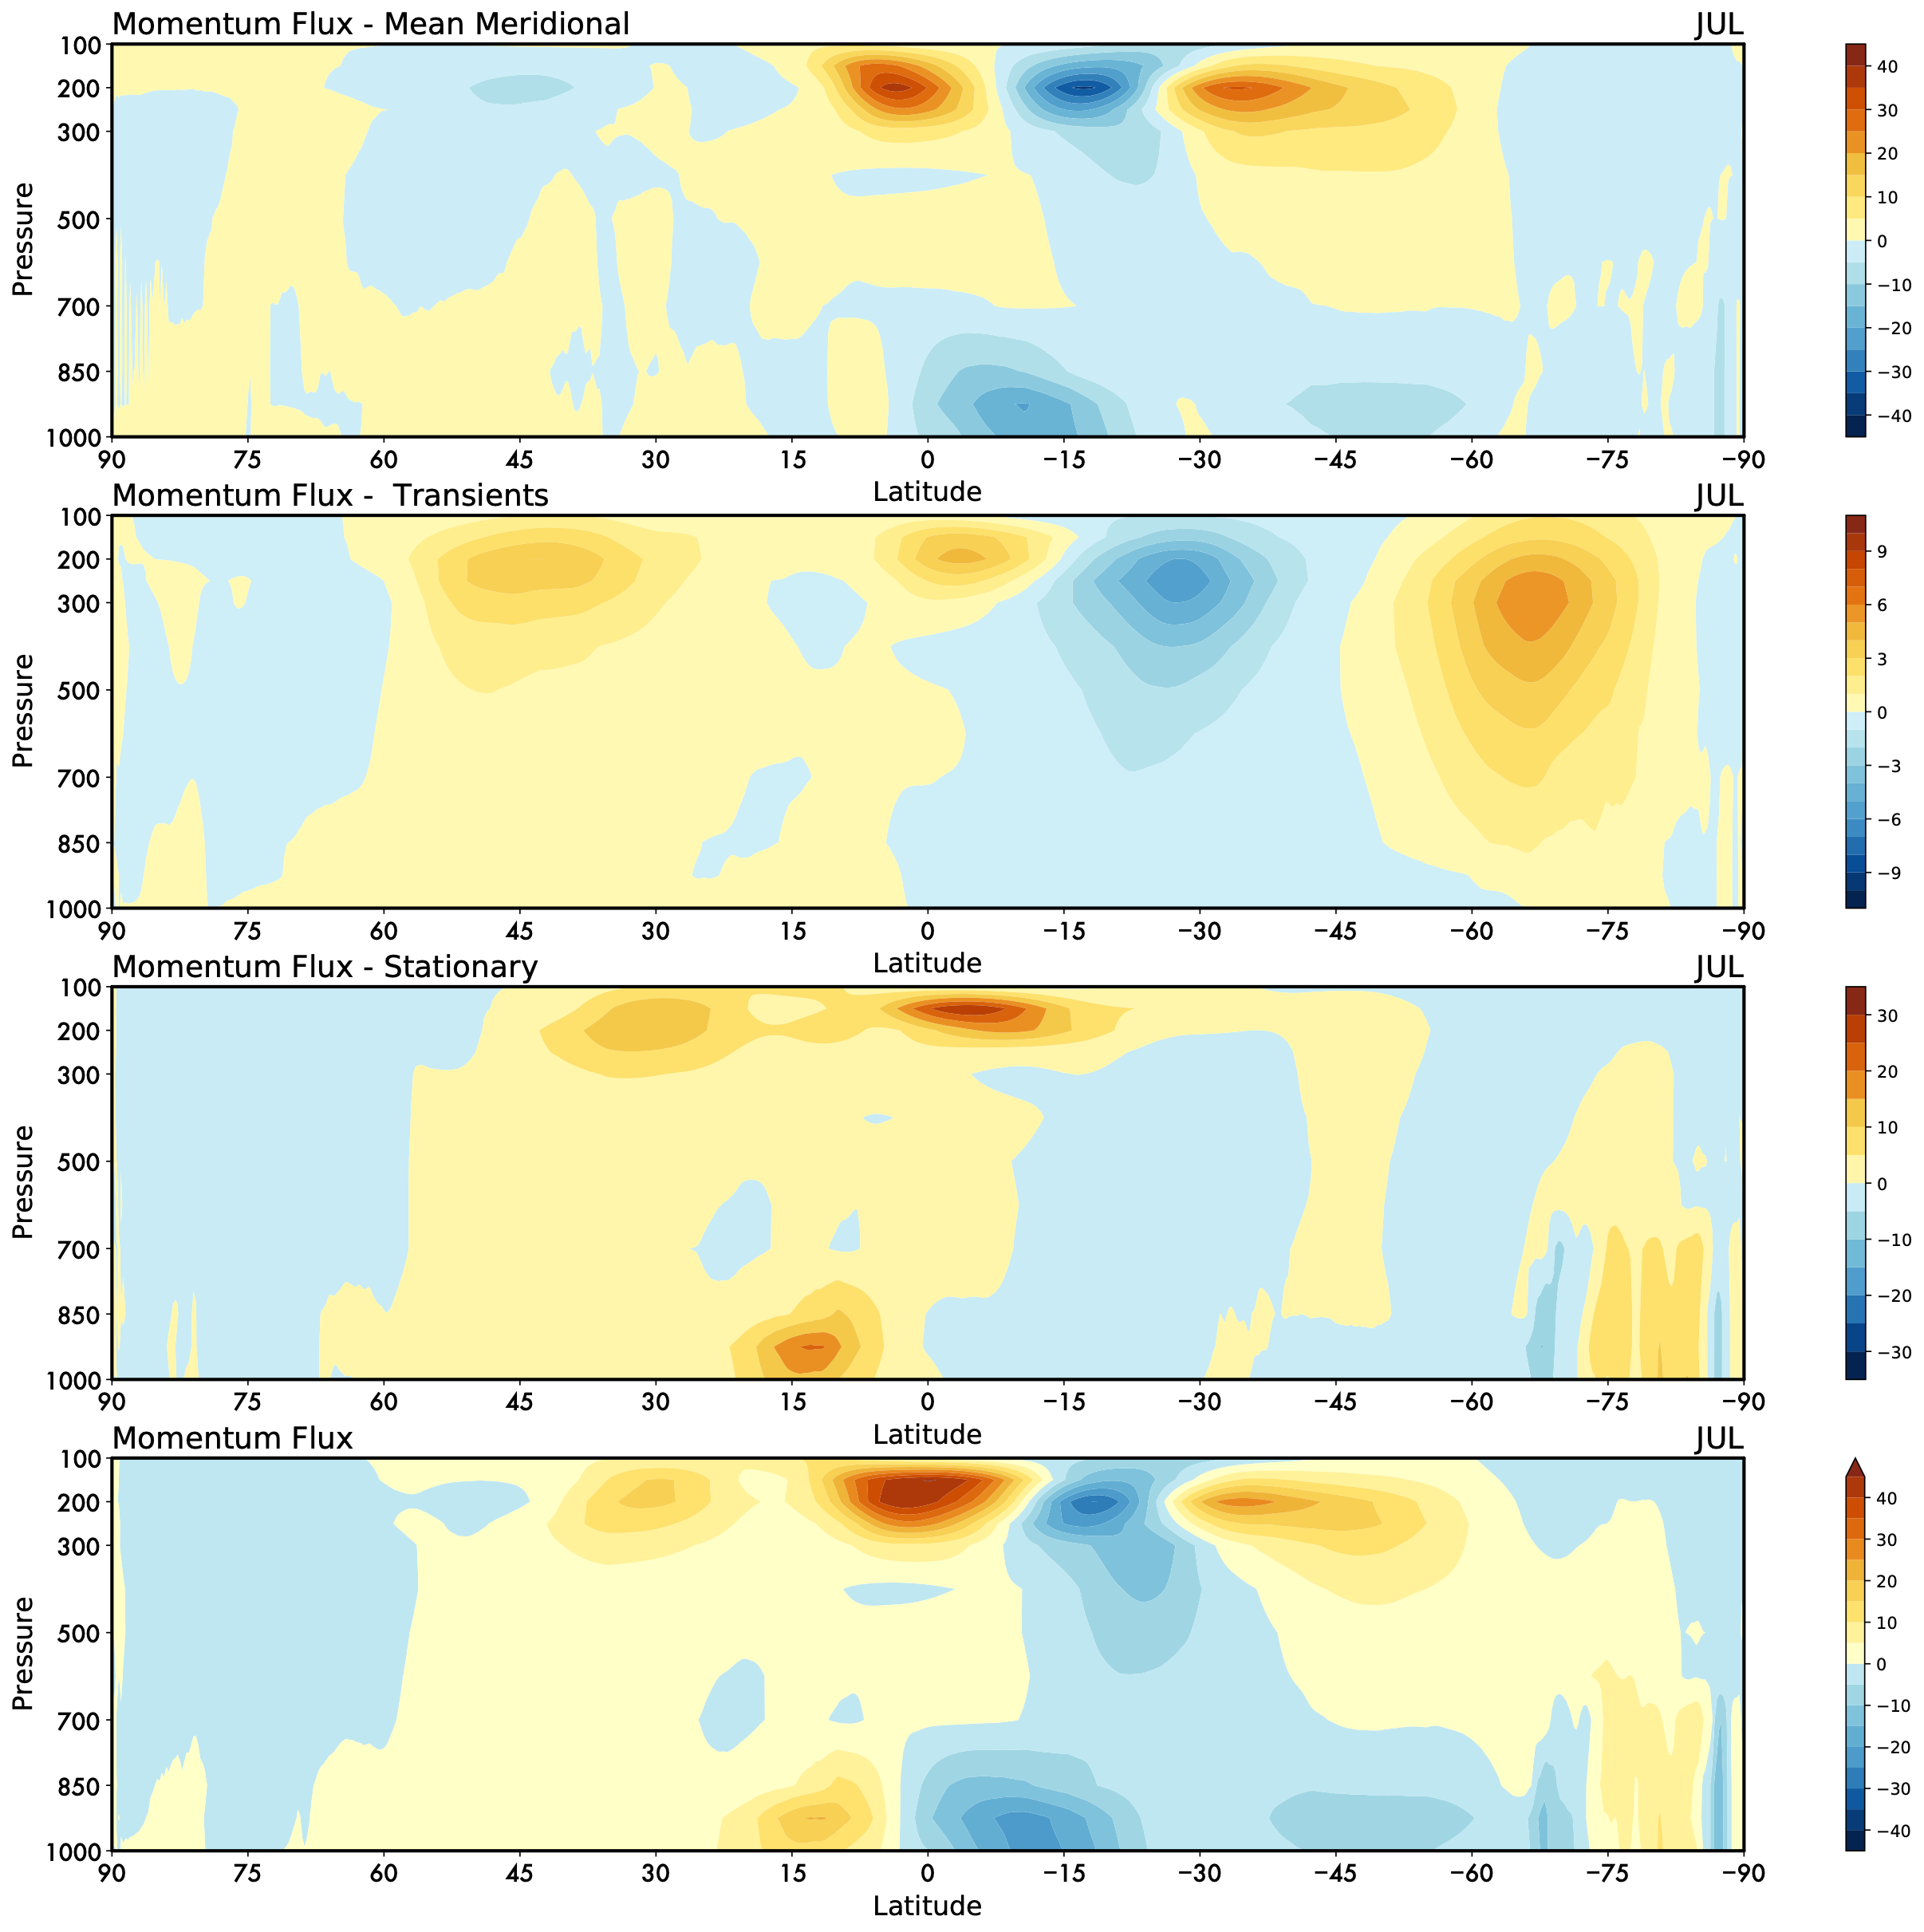
\includegraphics[width = .7 \textwidth]{figs/GD/JULUVFlux.png}
\caption{}\label{}
\end{figure}

\subsection{The Meridional Heat Flux}\label{the-meridional-heat-flux}

\begin{figure}
\centering
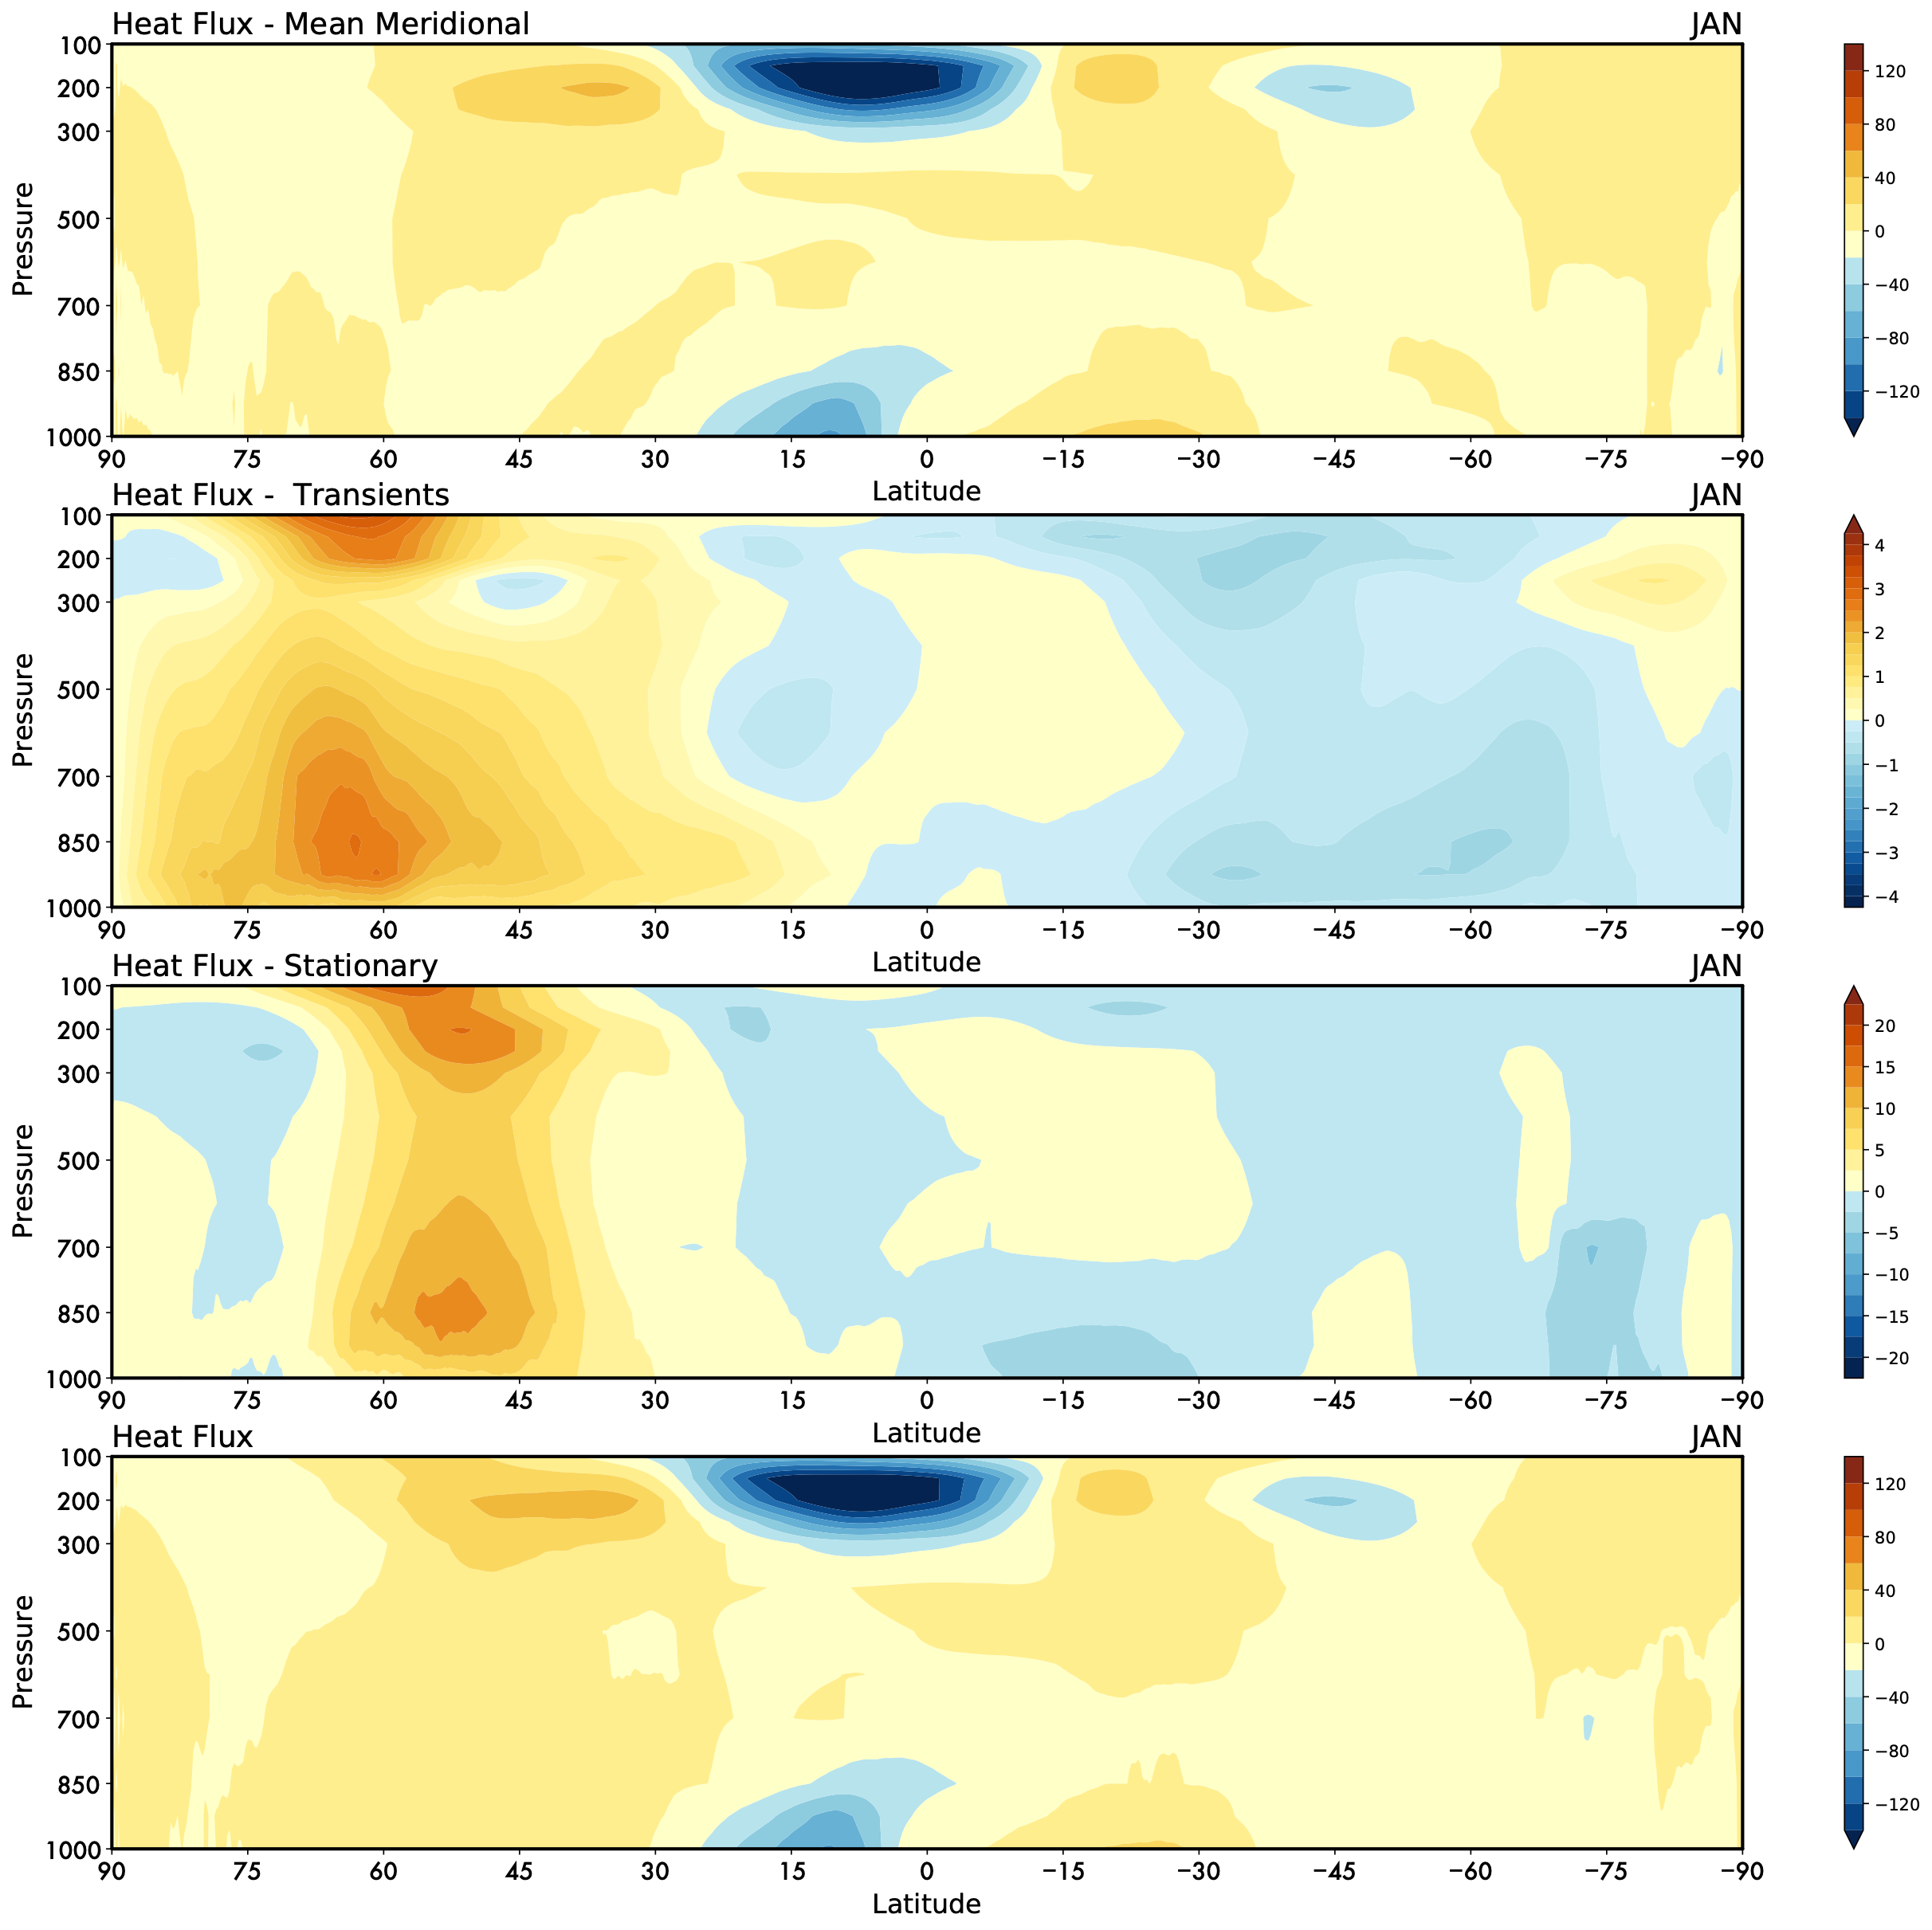
\includegraphics[width = .7 \textwidth]{figs/GD/JANTVFlux.png}
\caption{}\label{}
\end{figure}

\begin{figure}
\centering
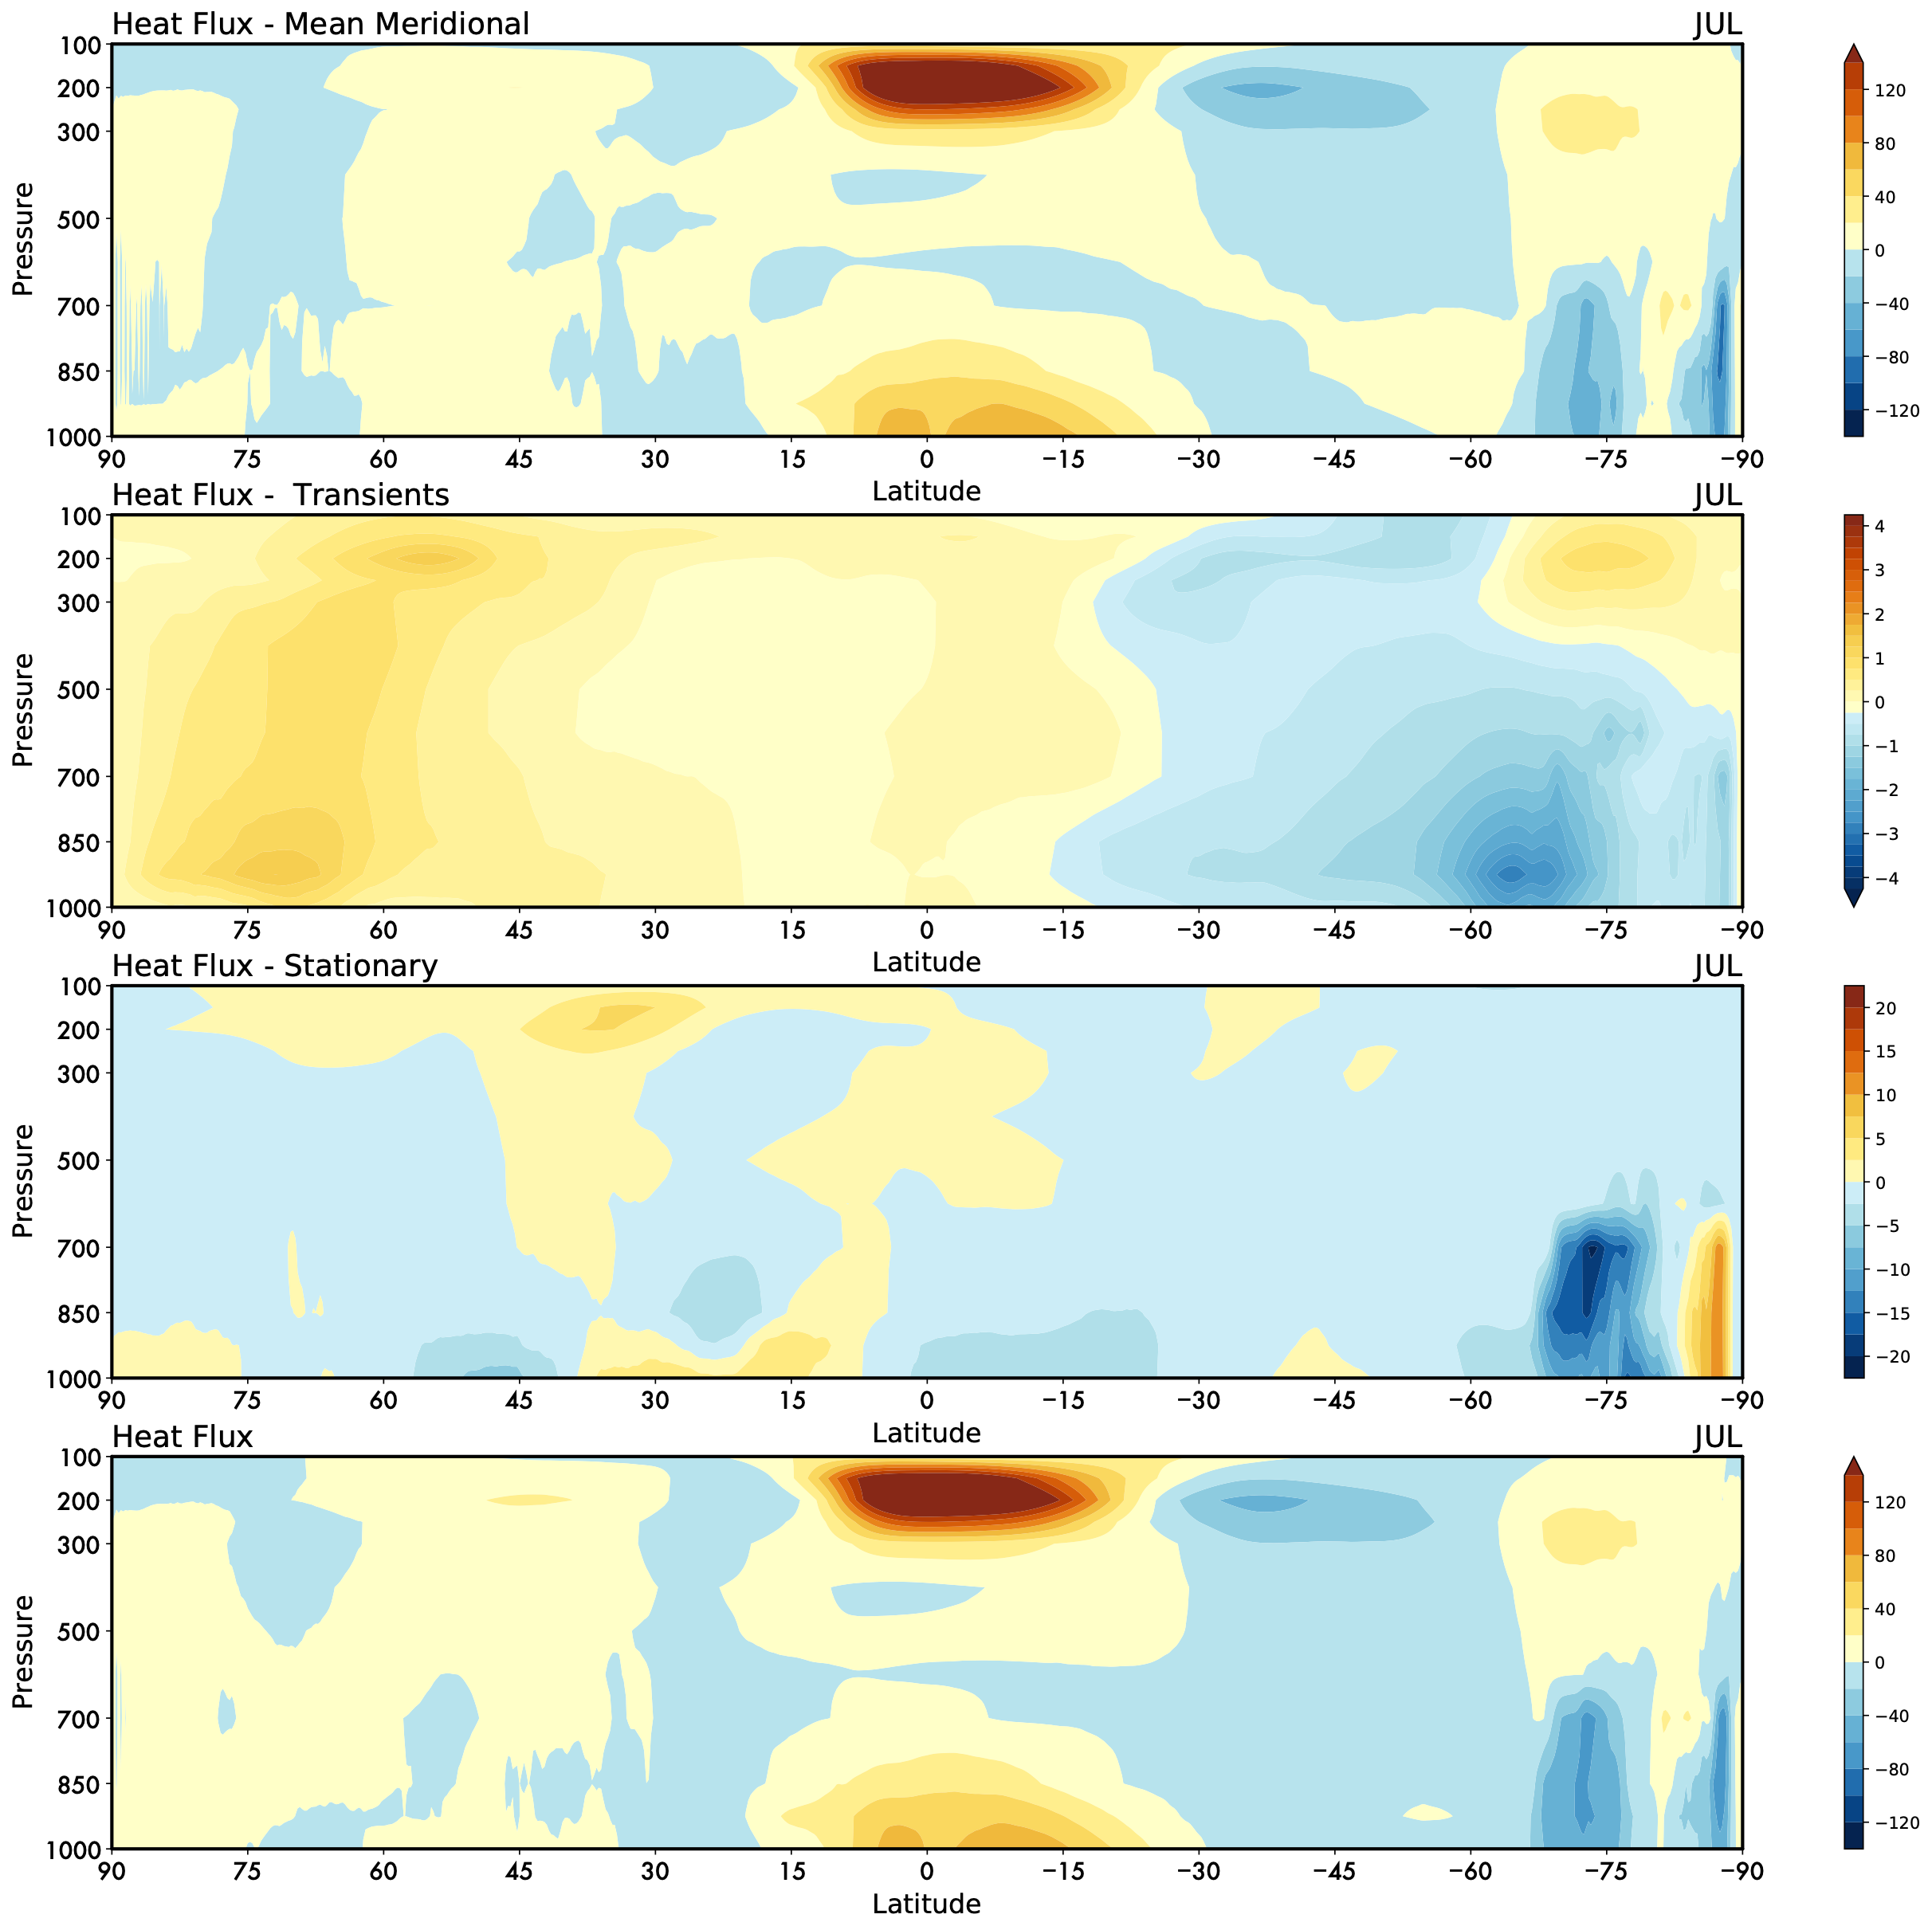
\includegraphics[width = .7 \textwidth]{figs/GD/JULTVFlux.png}
\caption{}\label{}
\end{figure}

The seasonal picture are in the appendix
